\documentclass[preprint,nocopyrightspace]{sigplanconf}

\pagestyle{plain}
\usepackage{balance,pfsteps}
\usepackage{aliascnt}
\usepackage{amsmath,stmaryrd,natbib,listings,graphicx,amsthm,amssymb,mathpartir,mnsymbol}
\usepackage[usenames,dvipsnames]{color}

\newcommand{\Scribtexttt}[1]{{\texttt{#1}}}
\newcommand{\SColorize}[2]{\color{#1}{#2}}
\newcommand{\inColor}[2]{{\Scribtexttt{\SColorize{#1}{#2}}}}
\definecolor{PaleBlue}{rgb}{0.90,0.90,1.0}
\newcommand{\rackett}[1]{\inColor{black}{#1}}
\newcommand{\todo}[1]{\textbf{TODO:} #1}
\newcommand{\iftr}[1]{#1}

\newcommand{\eg}{\textit{e.g.}}
\newcommand{\ie}{\textit{i.e.}}

\newcommand{\nat}{{\mathbb N}}
% Metavariables from defined spaces
\newcommand{\mexpr}{e}
\newcommand{\mexpri}[1]{e_{#1}}
\newcommand{\mvar}{x}
\newcommand{\mval}{v}
\newcommand{\mvalpre}{v_\mathit{pre}}
\newcommand{\mvalpost}{v_\mathit{post}}
\newcommand{\mtag}{v_{\mathit{t}}}
\newcommand{\mhandler}{v_\mathit{h}}
\newcommand{\maddr}{a}
\newcommand{\maddralt}{b}
\newcommand{\menv}{\rho}
\newcommand{\mstore}{\sigma}
\newcommand{\mkont}{\kappa}
\newcommand{\mskont}{\hat{\kappa}}
\newcommand{\mmkontacc}{C_\mathit{acc}}
\newcommand{\mmkont}{C}
\newcommand{\mstate}{\varsigma}
\newcommand{\mastate}{\hat\varsigma}

\newcommand{\mtime}{t}
\newcommand{\mtimealt}{u}

\newcommand{\mmarks}{m}
\newcommand{\mmarkset}{\chi}
\newcommand{\mprim}{\mathit{prim}}

\newcommand{\mktab}{\Xi}
\newcommand{\mmktab}{\chi}
\newcommand{\mmemo}{M}
\newcommand{\mpoint}{p}
\newcommand{\mctx}{\mathit{ctx}}
\newcommand{\msctx}{\mathit{vctx}}
\newcommand{\mframe}{\xi}
\newcommand{\mkframe}{\phi}
\newcommand{\mlab}{\ell}
\newcommand{\mtrace}{\pi}

\newcommand{\callcc}{\rackett{call/cc}}
\newcommand{\callcomp}{\rackett{call/comp}}
\newcommand{\abort}{\rackett{abort}}
\newcommand{\dynamicwind}{\rackett{dynamic-wind}}

% Metavariables for Spaces
\newcommand{\CEK}{\mathit{CEK}}
\newcommand{\CESKstart}{\mathit{CESK^*_t}}

\newcommand{\Var}{\mathit{Var}}

\newcommand{\Addr}{\mathit{Addr}}
\newcommand{\Time}{\mathit{Time}}

\newcommand{\Expr}{\mathit{Expr}}
\newcommand{\Store}{\mathit{Store}}
\newcommand{\Kont}{\mathit{Kont}}
\newcommand{\SKont}{\widehat{\mathit{Kont}}}
\newcommand{\MKont}{\mathit{MKont}}
\newcommand{\Env}{\mathit{Env}}
\newcommand{\State}{\mathit{State}}
\newcommand{\System}{\mathit{System}}
\newcommand{\Value}{\mathit{Value}}
\newcommand{\Prims}{\mathit{Prims}}

\newcommand{\maenv}{\hat{\menv}}
\newcommand{\makont}{\hat{\mkont}}

\newcommand{\Context}{\mathit{Context}}
\newcommand{\SContext}{\mathit{VContext}}

\newcommand{\Point}{\mathit{Point}}
\newcommand{\Frame}{\mathit{Frame}}
\newcommand{\Marks}{\mathit{Marks}}
\newcommand{\Markset}{\mathit{Markset}}

\newcommand{\KTab}{\mathit{Stack}}
\newcommand{\MKTab}{\mathit{MStack}}
\newcommand{\Memo}{\mathit{Memo}}

% Other metavariables (metafunction names, etc)
\newcommand{\inject}{\mathit{inject}}

\newcommand{\alloc}{\mathit{alloc}}
\newcommand{\tick}{\mathit{tick}}

\newcommand{\bind}{{\mathcal B}}
\newcommand{\lookup}{{\mathcal L}}
\newcommand{\wn}{\mathit{wn}}
\newcommand{\dom}{\text{dom}}
\newcommand{\onep}{\mathit{One?}}
\newcommand{\reverse}{\mathit{reverse}}
\newcommand{\revapp}{\mathit{rev\text{-}append}}
\newcommand{\finalize}{\mathit{finalize}}
\newcommand{\captureupto}{\mathit{capture\text{-}upto}}
\newcommand{\aborttargets}{\mathit{abort\text{-}targets}}

\newcommand{\startstate}{\mathit{base}}
\newcommand{\tails}[2]{\mathit{tails}_{#1}(#2)}
\newcommand{\tailscont}[3]{\mathit{tails}_{#1}^{#2}(#3)}
\newcommand{\reify}{\mathit{reify}}
\newcommand{\reflect}{\mathit{reflect}}
\newcommand{\reachrestrict}{\mathit{unfold}}
\newcommand{\stepextend}{\mathit{unfold}_1}

\newcommand{\domark}{\mathit{mark}}
\newcommand{\domarkset}{\mathit{markset}}
\newcommand{\returns}{{\mathbb R}}
\newcommand{\memoize}{{\mathbb M}}
\newcommand{\approximate}{{\mathbb A}}
\newcommand{\touches}{{\mathcal T}}
\newcommand{\touchesf}{{\mathcal T}_{\mkframe}}
\newcommand{\touchesk}[1]{{\mathcal T}_{#1}}
\newcommand{\reaches}{{\mathcal R}}
\newcommand{\konts}{\mathit{konts}}

\newcommand{\inv}{\mathit{inv}}
\newcommand{\reachable}{\mathit{reach}}
\newcommand{\memo}{\mathit{memo}}
\newcommand{\unroll}[2]{\mathit{unroll}_{#1}(#2)}
\newcommand{\unrollK}[3]{\mathit{unrollK}^{#1}_{#2}(#3)}
\newcommand{\unrollC}[2]{\mathit{unrollC}_{#1}(#2)}
\newcommand{\hastail}{\mathit{ht}}
\newcommand{\replacetail}{\mathit{rt}}

\newcommand{\kontlive}{K{\mathcal L}{\mathcal L}}
\newcommand{\kontliveaux}{K{\mathcal L}{\mathcal L}^*}
\newcommand{\terminal}{\mathit{terminal}}
\newcommand{\terminalaux}{\mathit{terminal}^*}
\newcommand{\trystep}{\mathit{trystep}}
\newcommand{\post}{\mathit{post}}

% Constructors
\newcommand{\svar}[2][{}]{#2^{#1}}
\newcommand{\sapp}[3][{}]{(#2\ #3)#1}
\newcommand{\slam}[3][{}]{\lambda#1 #2. #3}
\newcommand{\sprim}[1]{#1}
\newcommand{\sreset}[1]{(\texttt{reset}\ #1)}
\newcommand{\sshift}[2]{(\texttt{shift}\ #1. #2)}

\newcommand{\swcm}[3]{(\texttt{wcm}\ #1\ #2\ #3)}
\newcommand{\sccms}{(\texttt{ccm})}
\newcommand{\scmsf}{\texttt{cms-first}}
\newcommand{\scmsl}[2]{(\texttt{cms->list}\ #1\ #2)}

\newcommand{\cons}[2]{(\texttt{cons}\ #1\ #2)}
\newcommand{\smarkset}[1]{(\texttt{mark-set}\ #1)}

\newcommand{\vcont}[1]{\mathbf{cont}(#1)}
\newcommand{\vcomp}[1]{\mathbf{comp}(#1)}
\newcommand{\vclo}[2]{(#1, #2)}
\newcommand{\kar}[2][{}]{\mathbf{ar}#1(#2)}
\newcommand{\kpush}[1]{\mathbf{push}(#1)}
\newcommand{\klet}[1]{\mathbf{lt}(#1)}
\newcommand{\kfn}[2][{}]{\mathbf{fn}#1(#2)}
\newcommand{\kwcm}[1]{\mathbf{km}(#1)}
\newcommand{\kwcmk}[1]{\mathbf{kw1}(#1)}
\newcommand{\kwcmv}[1]{\mathbf{kw2}(#1)}
\newcommand{\kcmsls}[1]{\mathbf{kset}(#1)}
\newcommand{\kcmslk}[1]{\mathbf{kkey}(#1)}

\newcommand{\appl}[1]{\mathbf{appL}(#1)}
\newcommand{\appr}[1]{\mathbf{appR}(#1)}


\newcommand{\rt}{\mathbf{rt}}
\newcommand{\krt}[1]{\rt(#1)}
\newcommand{\kmt}{\mathbf{mt}}

\newcommand{\kprompt}[1]{\#(#1)}
\newcommand{\dw}{\mathbf{dw}}
\newcommand{\kdw}[1]{\dw(#1)}
\newcommand{\abrt}{\mathbf{abrt}}
\newcommand{\kabrt}[1]{\abrt(#1)}
\newcommand{\kev}[1]{\mathbf{ev}(#1)}

\newcommand{\mextag}[4]{(\#^{#2}_{#3} #1\ #4)}
\newcommand{\kmatch}[4]{(?^{#2}_{#3} #1\ #4)}
\newcommand{\mkapp}[2]{#1\circ #2}

% Notations
\newcommand{\sa}[1]{\widehat{\mathit{#1}}}

\newcommand{\lfp}{\mathbf{lfp}}
\newcommand{\tpl}[1]{\langle #1 \rangle}
\newcommand{\vect}[1]{\langle #1 \rangle}
\newcommand{\runpost}[1]{\langle #1 \rangle_{\mathit{post}}}
\newcommand{\runhandler}[1]{\langle #1 \rangle_{\mathit{handler}}}
\newcommand{\cstate}[1]{\langle #1 \rangle_{\mathit{call}}}
\newcommand{\set}[1]{\{ #1 \}}
\newcommand{\setbuild}[2]{\{ #1\ :\ #2\}}
\newcommand{\setbuildb}[2]{\left\{ #1\ :\ #2\right\}}
\newcommand{\nequiv}{\centernot\equiv}

\newcommand{\many}[1]{\overline{#1}}
\newcommand{\kcons}[2]{#1{\tt :} #2}
\newcommand{\alt}{\mathrel{\mid}}

\newcommand{\snglm}[2]{[#1 \mapsto \set{#2}]}
\newcommand{\extm}[3]{#1[#2 \mapsto #3]}
\newcommand{\joinm}[3]{#1\sqcup[#2 \mapsto #3]}
\newcommand{\joinone}[3]{#1\sqcup[#2 \mapsto \set{#3}]}
\DeclareMathOperator*{\finto}{\rightharpoonup}
\DeclareMathOperator*{\deceq}{\overset{?}{=}}

\newcommand{\append}[2]{#1 {\tt ++} #2}

%% Relations
\newcommand{\stepto}{\longmapsto}
\newcommand{\pdstepto}{\longmapsto_{\mathit{\Xi{}M}}}
\newcommand{\astepto}{\mathrel{\widehat{\longmapsto}}}
\newcommand{\tred}[1]{\mathrel{\underset{\Pi}{#1}}}

\newcommand{\klectx}[3]{#2 \mathrel{\sqsubseteq_{#1}} #3}
\usepackage{centernot}
\newcommand{\SCodePreSkip}{\vskip\abovedisplayskip}
\newcommand{\SCodePostSkip}{\vskip\belowdisplayskip}
\newenvironment{SCodeFlow}{\SCodePreSkip\begin{list}{}{\topsep=0pt\partopsep=0pt%
\listparindent=0pt\itemindent=0pt\labelwidth=0pt\leftmargin=2ex\rightmargin=2ex%
\itemsep=0pt\parsep=0pt}\item}{\end{list}\SCodePostSkip}
\newenvironment{SingleColumn}{\begin{list}{}{\topsep=0pt\partopsep=0pt%
\listparindent=0pt\itemindent=0pt\labelwidth=0pt\leftmargin=0pt\rightmargin=0pt%
\itemsep=0pt\parsep=0pt}\item}{\end{list}}
\newenvironment{RktBlk}{}{}
\definecolor{IdentifierColor}{rgb}{0.15,0.15,0.50}
\definecolor{ParenColor}{rgb}{0.52,0.24,0.14}
\newcommand{\RktSym}[1]{\inColor{IdentifierColor}{#1}}
\newcommand{\RktPn}[1]{\inColor{ParenColor}{#1}}

\newcommand{\Stttextless}{{\fontencoding{T1}\selectfont<}}
\definecolor{ValueColor}{rgb}{0.13,0.55,0.13}
\newcommand{\RktVal}[1]{\inColor{ValueColor}{#1}}

\newcommand{\ifwcm}[1]{}

\newtheorem{theorem}{Theorem}  
 
\newaliascnt{lemma}{theorem}  
\newtheorem{lemma}[lemma]{Lemma}  
\aliascntresetthe{lemma}  
\providecommand*{\lemmaautorefname}{Lemma}

\title{Abstracting Abstract Control}
\authorinfo{J. Ian Johnson}{Northeastern University}{ianj@ccs.neu.edu}
\authorinfo{David Van Horn}{University of Maryland}{dvanhorn@cs.umd.edu}

\usepackage{hyperref}
\begin{document}
\maketitle

% Outline:
% Introduction.
% High level
% PDCFA
% - Concrete
% - Abstract
% CFA2
% - Concrete
% - Abstract
% WCM machine
% - Concrete
% - Abstract
% Related Work
% Future Work
% Conclusion

\begin{abstract}
The strength of a dynamic language is also its weakness: run-time
flexibility comes at the cost of compile-time predictability.
%
Many of the hallmarks of dynamic languages such as closures,
continuations, various forms of reflection, and a lack of static types
make many programmers rejoice, while compiler writers, tool
developers, and verification engineers lament.
%
The dynamism of these features simply confounds statically reasoning
about programs that use them.
%
Consequently, static analyses for dynamic languages are few, far
between, and seldom sound.

The ``abstracting abstract machines'' (AAM) approach to constructing
static analyses has recently been proposed as a method to ameliorate
the difficulty of designing analyses for such language features.
%
The approach, so called because it derives a function for the sound
and computable approximation of program behavior starting from the
abstract machine semantics of a language, provides a viable approach
to dynamic language analysis since all that is required is a machine
description of the interpreter.


The AAM recipe as originally described produces finite state
abstractions: the behavior of a program is approximated as a finite
state machine.
%
Such a model is inherently imprecise with it comes to reasoning about
the control stack of the interpreter: a finite state machine cannot
faithfully represent a stack.
%
Recent advances have shown that higher-order programs can be
approximated with pushdown systems.
%
However, such models, founded in automata theory, either breakdown or
require significant engineering in the face of dynamic language
features that inspect or modify the control stack.

In this paper, we tackle the problem of bringing pushdown flow
analysis to the domain of dynamic language features.  We revise the
abstracting abstract machines technique to target the stronger
computational model of pushdown systems.
%
In place of automata theory, we use only abstract machines and
memoization.
%
As case studies, we show the technique applies to a language with
closures, garbage collection, stack-inspection, and first-class
composable continuations.

\end{abstract}

\section{Introduction}
Good static analyses use a combination of abstraction techniques, economical data structures, and a lot of engineering~\citep{dvanhorn:CousotEtAl-TASE07,ianjohnson:DBLP:journals/ipl/YiCKK07}.
%
The cited exemplary works stand out from a vast amount of work attacking the problem of statically analyzing languages like C.
%
Dynamic languages do not yet have such gems.
%
The problem space is different, bigger, and full of new challenges.
%
The traditional technique of pushing abstract values around a graph to get an analysis will not work.
%
The first problem we must solve is, ``what graph?'' as control-flow is now part of the problem domain.
%
Second, features like stack inspection and first-class continuations are not easily shoe-horned into a CFG representation of a program's behavior.
%
% We need a new approach. % before heavily investing in engineering effort.

%
Luckily, there is an alternative to the CFG approach to analysis construction that is based instead on abstract machines, which are one step away from interpreters; they are interderivable in several instances~\citep{dvanhorn:Danvy:DSc}.
%
This alternative, called abstracting abstract machines
(AAM)~\citep{dvanhorn:VanHorn2012Systematic}, is a simple
idea that is generally applicable to even the most dynamic of
languages, \eg{},
JavaScript~\citep{ianjohnson:DBLP:journals/corr/KashyapDKWGSWH14}.
%
A downside is that all effective instantiations of AAM are finite state approximations.
%
Finite state techniques cannot precisely predict where a method or function call will return.
%
Dynamic languages have more sources for imprecision than non-dynamic languages (\eg{}, reflection, computed fields, runtime linking, {\tt eval}) that all need proper treatment in the abstract.
%
If we can't have precision in the presence of statically unknowable behavior, we should at least be able to \emph{contain} it in the states it actually affects.
%
Imprecise control flow due to finite state abstractions is an unacceptable containment mechanism.
%
It opens the flood gate to imprecision flowing everywhere through analyses' predictions.
%
It is also a solvable problem.
%

%
We extend the AAM technique to computably handle infinite state spaces by adapting pushdown abstraction methods to abstract machines.
%
The unbounded stack of pushdown systems is the mechanism to precisely match calls and returns.
%
We demonstrate the essence of our pushdown analysis construction by
first applying the AAM technique to a call-by-value functional
language (\S\ref{sec:aam}) and then revising the derivation to
incorporate an exact representation of the control stack
(\S\ref{sec:pushdown}).  We then show how the approach scales to
stack-reflecting language features such as garbage collection and
stack inspection (\S\ref{sec:inspection}), and stack-reifying features
in the form of first-class delimited control operators (\S\ref{sec:delim}).
%
These case studies show that the approach is robust in the presence of
features that need to inspect or alter the run-time stack, which
previously have required significant technical
innovations~\cite{dvanhorn:Vardoulakis2011Pushdown,ianjohnson:DBLP:journals/jfp/JohnsonSEMH14}.

Our approach appeals to operational intuitions rather than automata theory to justify the approach.
%
The intention is that the only prerequisite to designing a pushdown
analysis for a dynamic language is some experience with implementing
interpreters. %; not with automata theory or abstract domains.
%
%% By simplifying the technical approach and broadening both the audience
%% and applicability of pushdown analyses, we hope to enable progress
%% towards technical feats like
%% Astr\'ee~\citep{dvanhorn:CousotEtAl-TASE07}
%% for expressive, dynamic languages.
%
% The large problem domain of analyzing dynamic languages needs an army to tackle it, and we believe that AAM can feed that army.

\section{The AAM methodology}
\label{sec:aam}
Abstracting abstract machines is founded on three ideas:
\begin{enumerate}
\item{Recursive data structures are easily representable via indirection at recursive points. For example, the tail of a list goes from being a list to an address of a list in a heap.}
\item{A finite pool of addresses then means a finite state space}
\item{Reused addresses mean the heap must use weak updates: $[a \mapsto v]\sqcup[a \mapsto v'] = [a \mapsto \set{v,v'}]$ and non-deterministic lookups.}
\end{enumerate}

Concretely, let us consider an abstract machine for the call-by-value untyped lambda calculus: the CEK machine.
%
The semantic spaces in \autoref{fig:cek-spaces} have three points of recursion: subexpressions, closures and pushed continuation frames.
%
The semantics for the CEK machine in \autoref{fig:cek-semantics} shows the delayed substitution semantics that environments enable.
%
Function application delays the substitution of an argument by extending the enviroment.
%
Variables dereference the environment to fulfill the delayed substitution semantics that the CEK machine implements.
%
Function application performs an administrative step to search for the next redex.
\begin{figure}\centering  
  \begin{align*}
    \mstate \in \CEK &::= \tpl{\mexpr, \menv, \mkont} \\
    \mexpr \in \Expr &::= \svar{\mvar} \alt \sapp{\mexpr}{\mexpr} \alt \mval \\
    \mval \in \Value &::= \slam{\mvar}{\mexpr} \\
    \menv \in \Env &= \Var \finto \Value \times \Env \\
    \mkframe \in \Frame &::= \appl{\mexpr,\menv} \alt \appr{\mval,\menv} \\
    \mkont \in \Kont &= \Frame^* \\
    \mvar \in \Var & \text{ an infinite space of variables}
  \end{align*}
  \caption{CEK semantic spaces}
\label{fig:cek-spaces}
\end{figure}

\begin{figure}
  \centering
  $\mstate \stepto \mstate'$ \\
  \begin{tabular}{r|l}
    \hline\vspace{-3mm}\\
    $\tpl{\svar\mvar, \menv, \mkont}$
    &
    $\tpl{\mval, \menv', \mkont}$ if $(\mval,\menv') = \menv(\mvar)$
    \\
% Application
    $\tpl{\sapp{\mexpri0}{\mexpri1},\menv,\mkont}$
    &
    $\tpl{\mexpri0,\menv,\kcons{\appl{\mexpri1,\menv}}{\mkont}}$
    \\
% Arg eval
    $\tpl{\mval,\menv, \kcons{\appl{\mexpr,\menv'}}{\mkont}}$
    &
    $\tpl{\mexpr,\menv',\kcons{\appr{\mval,\menv}}{\mkont}}$
    \\
% Function call
    $\tpl{\mval,\menv,\kcons{\appr{\slam{\mvar}{\mexpr},\menv'}}{\mkont}}$
    &
    $\tpl{\mexpr,\menv'[\mvar\mapsto(\mval,\menv)],\mkont}$
  \end{tabular}
  \caption{CEK machine}
  \label{fig:cek-semantics}
\end{figure}

The recursion in expressions is beneign because they are only destructed. The $\Expr$ space is finite for each program, the size of which is the number of subexpressions.
%
The run-away recursion is in $\Env$ and $\Kont$.
%
AAM suggests that the codomain of $\Env$\footnote{The strict criteria suggests $\Var \finto \Value \times \Addr$, but $\Var \finto \Addr$ is a sound approximation and relates more strongly to other analyses' approximations.} and the tail of the $\Frame$ list in $\Kont$ should instead be some $\Addr$ space.
%
Extensions to maps in $\Env$, and conses of frames in $\Kont$ then instead allocate an address, update the heap with the recursive value, and use the address in place of the recursive value.
%
To help an $\alloc : \State \to \Addr$ function choose its addresses, the state space can be extended with an arbitrary finite space that can be updated each step.
%
The original AAM paper calls this space and update function $\Time$ and $\tick$ respectively.
%
Later work on widening~\citep{ianjohnson:DBLP:conf/vmcai/HardekopfWCK14} suggests less arbitrary constructions, and to think of $\Time$ as a space of abstract traces, though the ``abstraction'' need not be sound~\citep{dvanhorn:Might2009Posteriori}.

The new semantic spaces in \autoref{fig:ceskstart-spaces} form the $\CESKstart$ machine.
%
We represent the machine differently than the original AAM paper to separate induced components (\eg{} the store and $\Time$) from transformed components (\eg{} the environment) for a uniform presentation.
%
The semantics of this machine follow the weak update and non-deterministic lookup principles of AAM in \autoref{fig:ceskstart-semantics}.

\begin{figure}
  \centering
  \begin{align*}
    \mstate \in \sa{CEK} &::= \tpl{\mexpr, \maenv, \makont} \\
    \sa{State} &= \sa{CEK} \times \Store \times \Time \\
    \mstore \in \Store &= \Addr \to \sa{Storeable} \\
    \menv \in \sa{Env} &= \Var \finto \Addr \\
    \mkont \in \sa{Kont} &::= \epsilon \alt \kcons{\mkframe}{\maddr} \\
    \sa{Storeable} &= \wp(\sa{Kont} + (\Value \times \sa{Env})) \\
    \maddr,\maddralt \in \Addr & \quad \mtime,\mtimealt \in \Time
  \end{align*}
  \caption{$\CESKstart$ semantic spaces}
  \label{fig:ceskstart-spaces}
\end{figure}

\begin{figure}
  \centering
  $\mstate,\mstore,\mtime \stepto \mstate',\mstore',\tick(\mstate,\mstore,\mtime)$ \quad $\maddr = \alloc(\mstate,\mstore,\mtime)$ \\
  \begin{tabular}{r|l}
    \hline\vspace{-3mm}\\
    $\tpl{\svar\mvar, \maenv, \makont}$
    &
    $\tpl{\mval, \maenv',\makont}$ if $(\mval,\menv') \in \mstore(\maenv(\mvar))$
    \\
% Application
    $\tpl{\sapp{\mexpri0}{\mexpri1},\maenv,\makont}$
    &
    $\tpl{\mexpri0,\maenv,\kcons{\appl{\mexpri1,\maenv}}{\maddr}}$ \\
    where & $\mstore' = \joinm{\mstore}{\maddr}{\makont}$
    \\
% Arg eval
    $\tpl{\mval,\maenv, \kcons{\appl{\mexpr,\maenv'}}{\maddralt}}$
    &
    $\tpl{\mexpr,\maenv',\kcons{\appr{\mval,\maenv}}{\maddralt}}$
    \\
% Function call
    $\tpl{\mval,\maenv,\kcons{\appr{\slam{\mvar}{\mexpr},\maenv'}}{\maddralt}}$
    &
    $\tpl{\mexpr,\maenv'',\makont}$ if $\makont \in \mstore(\maddralt)$ \\
    where & $\maenv'' = \maenv'[\mvar\mapsto\maddr]$ \\
          & $\mstore' = \joinm{\mstore}{\maddr}{(\mval,\maenv)}$
  \end{tabular} \\
  Where $\mstore' = \mstore$ unless otherwise stated.
  \caption{$\CESKstart$ semantics}
  \label{fig:ceskstart-semantics}
\end{figure}

If we run the $\CESKstart$ semantics to explore all possible states, we get a sound approximation of all paths that the $\CEK$ machine will explore.
%
The paper will give a more focused view of the $\Kont$ component.
%
Suppose a semantics that interacts with $\Kont$ via a stack discipline (only push and pop single frames at a time, \eg{} the above machine).
%
If we were not to heap-allocate the tail of a continuation, the resulting machine has all finite components except an unbounded stack of finitely many stack frames.
%
This is exactly a pushdown system.
%
We can exactly represent the stack and still have a sound and terminating analysis.
\section{A refinement for exact stacks}\label{sec:pushdown}
We can exactly represent the stack in the $\CESKstart$ machine with a modified allocation scheme for stacks.
%
The key idea is that if the address is ``precise enough,'' then every path that leads to the allocation will proceed exactly the same way until the address is dereferenced.
%

%
What constitutes ``precise enough''?
%
For the $\CESKstart$ machine, every function evaluates the same way, regardless of the stack.
%
We should then represent the stack addresses as the components of a function call.
%
The one place in the $\CESKstart$ machine that continuations are allocated is at $\sapp{\mexpri0}{\mexpri1}$ evaluation.
%
The expression itself, the environment, the store and the timestamp are necessary components for evaluating $\sapp{\mexpri0}{\mexpri1}$, so then we just represent the stack address as those four things.
%
The stack is not relevant for its evaluation, so we do not want to store the stack addresses in the same store -- that would also lead to a recursive heap structure.
%
We will call this new table $\mktab$, because it looks like a stack.
%

%
By not storing the continuations in the value store, we separate ``relevant'' components from ``irrelevant'' components.
%
We split the stack store from the value store and use only the value store in stack addresses.
%
Stack addresses generally describe the relevant context that lead to their allocation, so we will refer to them henceforth as \emph{contexts}.
%
The resulting state space is updated here:
  \begin{align*}
    \sa{State} &= \sa{CESK}_t \times \KStore \\
    \Storeable &= \Value \\
    \mkont \in \Kont &::= \epsilon \alt \kcons{\mkframe}{\mctx} \\
    \mctx \in \Context &::=  \tpl{\mexpr,\menv,\mstore}_\mtime \\
    \mktab \in \KStore &= \Context \finto \wp(\Kont) \\
  \end{align*}

The semantics is modified slightly in \autoref{fig:ceskkstart-semantics} to use $\mktab$ instead of $\mstore$ for continuation allocation and lookup.
%
Given finite allocation, contexts are drawn from a finite space, but are still precise enough to describe an unbounded stack.
%
The computed $\stepto$ relation thus represents the full description of a pushdown system of reachable states (and the set of paths).
%
Of course this semantics does not always define a pushdown system since $\alloc$ can have an unbounded codomain.
%
The correctness claim is therefore a correspondence between the same machine but with an unbounded stack, no $\mktab$, and $\alloc, \tick$ functions that behave the same disregarding the different representations (a reasonable assumption).

\begin{figure}
  \centering
  $\mastate,\mktab \stepto \mastate',\mktab'$ \quad $\maddr = \alloc(\mastate,\mktab)$ \quad $\mtimealt = \tick(\mastate,\mktab)$ \\
  \begin{tabular}{r|l}
    \hline\vspace{-3mm}\\
    $\tpl{\svar\mvar, \menv, \mstore, \makont}_\mtime,\mktab$
    &
    $\tpl{\mval, \mstore,\makont}_\mtimealt,\mktab$ if $\mval \in \mstore(\menv(\mvar))$
    \\
% Application
    $\tpl{\sapp{\mexpri0}{\mexpri1},\menv,\mstore,\makont}_\mtime,\mktab$
    &
    $\tpl{\mexpri0,\menv,\mstore,\kcons{\appl{\mexpri1,\menv}}{\mctx}}_\mtimealt,\mktab'$ \\
    where & $\mctx = \tpl{\sapp{\mexpri0}{\mexpri1},\menv,\mstore}_\mtime$ \\
          & $\mktab' = \joinm{\mktab}{\mctx}{\makont}$
    \\
% Arg eval
    $\tpl{\mval,\mstore,\kcons{\appl{\mexpr,\menv'}}{\mctx}}_\mtime,\mktab$
    &
    $\tpl{\mexpr,\menv',\mstore,\kcons{\appr{\mval}}{\mctx}}_\mtimealt,\mktab$
    \\
% Function call
    $\tpl{\mval,\menv,\mstore,\kcons{\appr{\slam{\mvar}{\mexpr},\menv'}}{\mctx}}_\mtime,\mktab$
    &
    $\tpl{\mexpr,\menv'',\mstore',\makont}_\mtimealt,\mktab$ if $\makont \in \mktab(\mctx)$ \\
    where & $\menv'' = \extm{\menv'}{\mvar}{\maddr}$ \\
          & $\mstore' = \joinm{\mstore}{\maddr}{\mval}$
  \end{tabular}
  \caption{$\CESKKstart$ semantics}
  \label{fig:ceskkstart-semantics}
\end{figure}

\subsection{Correctness}

The high level argument for correctness exploits properties of both machines.
%
Where the stack is unbounded (call this $\CESKt$), if every state in a trace shares a common tail in their continuations, that tail is \emph{irrelevant}.
%
This means the tail can be replaced with anything and still produce a valid trace.
%
We call this property more generally, ``context irrelevance.''
%
The $\CESKKstart$ machine maintains an invariant on $\mktab$ that says that $\makont \in \mktab(\mctx)$ represents a trace in $\CESKt$ that starts at the base of $\makont$ and reaches $\mctx$ with $\makont$ on top.
%
We can use this invariant and context irrelevance to translate steps in the $\CESKKstart$ machine into steps in $\CESKt$.
%
The other way around, we use a proposition that a full stack is represented by $\mktab$ via unrolling and follow a simple simulation argument.

The common tail proposition we will call $\hastail$ and the replacement function we will call $\replacetail$; they both have obvious inductive and recursive definitions respectively.
%
The invariant is stated with respect to the entire program, $\mexpr_\mathit{pgm}$:
\begin{mathpar}
  \inferrule{ }{\invmktab(\bot)} \quad
  \inferrule{\invmktab(\mktab) \\
      \forall \makont_c \in K. \startstate(\makont_c) \stepto_\CESKt^* \tpl{\mexpr_c,\menv_c,\mstore_c,\append{\mkont_c}{\epsilon}}_{\mtime_c}}
            {\invmktab(\extm{\mktab}{\tpl{\mexpr_c,\menv_c,\mstore_c}_{\mtime_c}}{K})} \\

  \inferrule{
    % invariant for current state
    \startstate(\makont) \stepto_\CESKt^* \tpl{\mexpr,\menv,\mstore,\append{\makont}{\epsilon}}_\mtime \\
    % invariant for all entries
    \invmktab(\mktab)}
    {\inv(\tpl{\mexpr,\menv,\mstore,\makont}_\mtime,\mktab)}
  \end{mathpar}
where
\begin{align*}
 \startstate(\epsilon) &= \tpl{\mexpr_\mathit{pgm},\bot,\bot,\epsilon}_{\mtime_0} \\
                \startstate(\kcons{\mkframe}{\tpl{\mexpr_c,\menv_c,\mstore_c}_{\mtime_c}}) &=
                \tpl{\mexpr_c,\menv_c,\mstore_c,\epsilon}_{\mtime_c}
\end{align*}
We use $\append{\cdot}{\epsilon}$ to treat $\mctx$ like $\epsilon$ and construct a continuation in $\Kont$ rather than $\sa{Kont}$.
%%
\begin{lemma}[Context irrelevance]\label{lem:irrelevance}
  For all traces $\mtrace \in \CESKt^*$ and continuations $\mkont$ such that $\hastail(\mtrace,\mkont)$, for any $\mkont'$, $\replacetail(\mtrace,\mkont,\mkont')$ is a valid trace.
\end{lemma}
\begin{proof}
  Simple induction on $\mtrace$ and cases on $\stepto_{\CESKt}$.
\end{proof}
\begin{lemma}[$\CESKKstart$ Invariant]\label{lem:invariant}
  For all $\mstate,\mstate' \in \sa{State}$, if $\inv(\mstate)$ and $\mstate \stepto \mstate'$, then $\inv(\mstate')$
\end{lemma}
\begin{proof}
  Routine case analysis.
\end{proof}
Note that the injection of $\mexpr_\mathit{pgm}$ into $\CESKKstart$, $(\tpl{\mexpr_\mathit{pgm},\bot,\bot,\epsilon}_{\mtime_0},\bot)$, trivially satisfies $\inv$.

The unrolling proposition is the following
\begin{mathpar}
  \inferrule{ }{\epsilon \in \unroll{\mktab}{\epsilon}} \quad
  \inferrule{\makont \in \mktab(\mctx),
             \mkont \in \unroll{\mktab}{\makont}}
            {\kcons{\mkframe}{\mkont} \in \unroll{\mktab}{\kcons{\mkframe}{\mctx}}}
\end{mathpar}
\begin{theorem}[Correctness]\label{thm:pushdown-correct}
  For all expressions $\mexpr_\mathit{pgm}$,
  \begin{itemize}
  \item{{\bf Soundness: } %for all $\mstate\equiv\tpl{\mexpr,\menv,\mkont},\mstate'\equiv{\mexpr',\menv',\mkont'} \in \CESKt$,
        if $\mstate \stepto_{\CESKt} \mstate'$,
        %for all $\mktab,\makont$ if
        $\inv(\mstate\set{\mkont := \makont},\mktab)$,
        and $\mkont \in \unroll{\mktab}{\makont}$, then
        there are $\mktab',\makont'$ such that
        $\mstate\set{\mkont := \makont},\mktab \stepto_{\CESKKstart} \mstate'\set{\mkont := \makont'},\mktab'$ and $\mkont' \in \unroll{\mktab'}{\makont'}$}
  \item{{\bf Completeness:} if $\mastate,\mktab \stepto_{\CESKKstart} \mastate',\mktab'$
      and $\inv(\mastate,\mktab)$,
      for all $\mkont$, if $\mkont \in \unroll{\mktab}{\mastate.\makont}$ then
      there is a $\mkont'$ such that
      $\mastate\set{\makont := \mkont} \stepto_{\CESKt}
       \mastate'\set{\makont := \mkont'}$ and
       $\mkont' \in \unroll{\mktab}{\mastate'.\makont}$.}
  \end{itemize}
\end{theorem}

\subsection{Engineered semantics for efficiency}\label{sec:eng-frontier}
%%
We cover three optimizations that may be employed to accelerate the fixed-point computation.
\begin{enumerate}
\item{Observe that $\mktab$ can be made global with no loss in precision; it will not need to be stored in the frontier or set of seen states.}
\item{\label{item:chunk}Continuations can be ``chunked'' more coarsely at function boundaries instead of at each frame in order to minimize table lookups.}
\item{Since evaluation is the same regardless of the stack, we can memoize results to short-circuit to the answer.}
\end{enumerate}
%
This last optimization will be covered in more detail in \autoref{sec:memo}.
%
From here on, this paper will not explicitly mention timestamps.

A secondary motivation for the representation change in \ref{item:chunk} is that flow analyses commonly split control-flow graphs at function call boundaries to enable the combination of intra- and inter-procedural analyses.
%
In an abstract machines, this split looks like installing a continuation prompt at function calls.
%
We borrow a representation from literature on delimited continuations~\citep{ianjohnson:Biernacki2006274} to split the continuation into two components: the continuation and meta-continuation.
%
Our delimiters are special since each continuation ``chunk'' until the next prompt has bounded length.
%
The bound is roughly the deepest nesting depth of an expression in functions' bodies.
%
Instead of ``continuation'' and ``meta-continuation'' then, we will use terminology from CFA2 and call the top chunk a ``local continuation,'' and the rest the ``continuation.''\footnote{Since the continuation is either $\epsilon$ or a context, CFA2 calls these ``entries'' to mean execution entry into the program ($\epsilon$) or a function ($\mctx$). One can also understand these as entries in a table ($\mktab$). We stay with the ``continuation'' nomenclature because they represent full continuations.}
%
%

\begin{figure}
  \centering
  \begin{tabular}{rlrl}
    $\mastate \in \sa{CESIK}$ &\hspace{-3mm}$= \tpl{\mexpr,\menv,\mstore,\mlkont,\makont}$& $\mlkont \in \LKont$ &\hspace{-3mm}$= \Frame^*$ \\
    & & $\makont \in \Kont$ &\hspace{-3mm}$::= \epsilon \alt \mctx$
  \end{tabular}
  \caption{$\CESIKKstart$ semantic spaces}
  \label{fig:pushdown-spaces}
\end{figure}

The resulting shuffling of the semantics to accommodate this new representation is in \autoref{fig:cesikkstart-semantics}.
%
The extension to $\mktab$ happens in a different rule -- function entry -- so the shape of the context changes to hold the function, argument, and store.
%
We have a choice of whether to introduce an administrative step to dereference $\mktab$ once $\mlkont$ is empty, or to use a helper metafunction to describe a ``pop'' of both $\mlkont$ and $\mkont$.
%
Suppose we choose the second because the resulting semantics has a 1-to-1 correspondence with the previous semantics.
%
A first attempt might land us here:
\begin{align*}
  \pop(\kcons{\mkframe}{\mlkont},\makont,\mktab) &= \set{(\mkframe,\mlkont,\makont)} \\
  \pop(\epsilon,\mctx,\mktab) &= \setbuild{(\mkframe,\mlkont,\makont)}{(\kcons{\mkframe}{\mlkont}, \makont) \in \mktab(\mctx)}
\end{align*}
However, tail calls make the dereferenced $\mctx$ lead to $(\epsilon,\mctx')$.
%
Because abstraction makes the store grow monotonically in a finite space, it's possible that $\mctx' = \mctx$ and a naive recursive definition of $\pop$ will diverge chasing these contexts.
%
Now $\pop$ must save all the contexts it dereferences in order to guard against divergence.
%
So $\pop(\mlkont,\makont,\mktab) = \popaux(\mlkont,\makont,\mktab,\emptyset)$ where
\begin{align*}
  \popaux(\epsilon,\epsilon,\mktab,G) &= \emptyset \\
  \popaux(\kcons{\mkframe}{\mlkont},\makont,\mktab,G) &= \set{(\mkframe,\mlkont,\makont)} \\
  \popaux(\epsilon,\mctx,\mktab,G) &= \setbuild{(\mkframe,\mlkont,\makont)}{(\kcons{\mkframe}{\mlkont}, \makont) \in \mktab(\mctx)} \\
  &\cup \bigcup\limits_{\mctx' \in G'}\popaux(\epsilon,\mctx',\mktab,G\cup G') \\
  \text{where } G' &= \setbuild{\mctx'}{(\epsilon,\mctx') \in \mktab(\mctx)} \setminus G
\end{align*}

In practice, one would not expect $G$ to grow very large.
%
Had we chosen the first strategy, the issue of divergence is delegated to the machinery from the fixed-point computation.\footnote{CFA2 employs the first strategy and calls it ``transitive summaries.''}
%
However, when adding the administrative state, the ``seen'' check requires searching a far larger set than we would expect $G$ to be.

\begin{figure}
  \centering
  $\mastate,\mktab \stepto \mastate',\mktab'$ \quad $\maddr = \alloc(\mastate,\mktab)$ \\
  \begin{tabular}{r|l}
    \hline\vspace{-3mm}\\
    $\tpl{\svar\mvar, \menv, \mstore, \mlkont, \makont},\mktab$
    &
    $\tpl{\mval,\mstore,\mlkont,\makont},\mktab$ if $\mval \in \mstore(\menv(\mvar))$
    \\
% Application
    $\tpl{\sapp{\mexpri0}{\mexpri1},\menv,\mstore,\mlkont,\makont},\mktab$
    &
    $\tpl{\mexpri0,\menv,\mstore,\kcons{\appl{\mexpri1,\menv}}{\mlkont},\makont},\mktab$
    \\
% Arg eval
    $\tpl{\mval, \mstore, \mlkont,\makont},\mktab$
    &
    $\tpl{\mexpr,\menv',\mstore,\kcons{\appr{\mval,\menv}}{\mlkont'},\makont'},\mktab$ \\
    &
    if $\appl{\mexpr,\menv'},\mlkont',\makont' \in \pop(\mlkont,\makont,\mktab)$ \\
% Function call
    $\tpl{\mval,\mstore, \mlkont,\makont},\mktab$
    &
    $\tpl{\mexpr,\extm{\menv}{\mvar}{\maddr},\mstore',\epsilon,\mctx},\mktab'$ \\
    & if $\appr{\slam{\mvar}{\mexpr},\menv}, \mlkont', \makont' \in \pop(\mlkont,\makont,\mktab)$ \\
    where & $\mstore' = \joinm{\mstore}{\maddr}{\mval}$ \\
    & $\mctx = (\tpl{\slam{\mvar}{\mexpr},\menv},\mval,\mstore)$ \\
    & $\mktab' = \joinm{\mktab}{\mctx}{(\mlkont,\makont)}$
  \end{tabular} \\
  \caption{$\CESIKKstart$ semantics}
  \label{fig:cesikkstart-semantics}
\end{figure}

\begin{align*}
  {\mathcal F}_{\mexpr}(S,R,F,\mktab) &= (S \cup F, R \cup R', F'\setminus S, \mktab') \\
  I &= \bigcup\limits_{s=(\mastate,\mstore) \in F}{\setbuild{(\tpl{\mastate,\mastate'}, \mktab')}{\mastate,\mktab \stepto \mastate',\mktab'}} \\
  R' &= \pi_0 I \qquad F' = \pi_1 R' \qquad \mktab' = \bigsqcup\pi_1 I
\end{align*}
For a program $\mexpr$, we will say $(\emptyset,\emptyset,\set{\tpl{\mexpr,\bot,\bot,\epsilon,\epsilon}},\bot)$ is the bottom element of ${\mathcal F}_{\mexpr}$'s domain.
%
The ``analysis'' then is then the pair of the $R$ and $\mktab$ components of $\lfp({\mathcal F}_{\mexpr})$.

The correctness argument for this semantics is not about single steps but instead about the entire relation that ${\mathcal F}$ computes.
%
The argument is that the $R$ and $\mktab$ components of the system represent a slice of the unbounded relation $\stepto_{\CESK}$ (restricted to reachable states).
%
We will show that traces in any $n \in \nat$ times we \emph{unfold} $\stepto_{\CESK}$ from the initial state, there is a corresponding $m$ applications of ${\mathcal F}$ that reify into a relation that exhibit the same trace.
%
Conversely, any trace in the reification of ${\mathcal F}_{\mexpr}^m(\bot)$ has the same trace in some $n$ unfoldings of $\stepto_{\CESK}$.
%
For an arbitrary $\alloc$ function, we cannot expect ${\mathcal F}$ to have a fixed point, so this property is the best we can get.
%
For a finite $\alloc$ function, Kleene's fixed point theorem dictates there is a $m$ such that ${\mathcal F}_{\mexpr}^m(\bot)$ is a fixed point, so every trace in the reified relation is also a trace in an unbounded number of unfoldings of $\stepto_{\CESK}$.
%
This is the corresponding completeness argument for the algorithm.

\begin{align*}
  \reachrestrict(\mstate_0, \stepto, 0) &= \setbuild{(\mstate_0,\mstate)}{\mstate_0 \stepto \mstate} \\
  \reachrestrict(\mstate_0, \stepto, n+1) &= \stepextend(\reachrestrict(\mstate_0,\stepto,n)) \\
  \textit{where } \stepextend(R) &= R \cup \setbuild{(\mstate,\mstate')}{(\_,\mstate) \in R, \mstate \stepto \mstate'}
\end{align*}
The reification simply realizes all possible complete continuations that a state could have, given $\mktab$:
\begin{mathpar}
  \inferrule{
  \tpl{\tpl{\mexpr,\menv,\mstore,\makont},
      \tpl{\mexpr',\menv',\mstore',\makont'}} \in R \\
  \mkont \in \tails{\mktab}{\makont}}
  {\tpl{\mexpr,\menv,\mstore,\append{\makont}{\mkont}} \stepto_{\reify(S,F,R,\mktab)}
   \tpl{\mexpr',\menv',\mstore'\append{\makont'}{\mkont}}}
  % \reify(S,F,R,\mktab) &= \setbuild{}
  % {\\ &\phantom{= \{}
  %   \tpl{(\tpl{\mexpr,\menv,\makont},\mstore,\mtime),
  %     (\tpl{\mexpr',\menv',\makont'},\mstore',\mtime')} \in R,
  %   \\ &\phantom{= \{}
  %   \mkont \in \tails{\mktab}{\makont}}
\end{mathpar}
The additional judgment about tails is a variant of $\mathit{unroll}$ in order to get a common tail:
\begin{mathpar}
  \inferrule{ }{\epsilon \in \tails{\mktab}{\epsilon}} \quad
  \inferrule{\makont \in \mktab(\mctx) \\
             \mkont \in \unroll{\mktab}{\makont}}
            {\mkont \in \tails{\mktab}{\kcons{\mkframe}{\mctx}}}
\end{mathpar}
\begin{theorem}[Correctness]\label{thm:global-pushdown}
  For all $\mexpr_0$, let $\mstate_0 = \tpl{\mexpr_0,\bot,\bot,\epsilon}$ in
  $\forall n \in \nat, \mstate,\mstate' \in \CESK$:
  \begin{itemize}
  \item{if $(\mstate,\mstate') \in \reachrestrict(\mstate_0,\stepto_{\CESK},n)$ then
      there is an $m$ such that $\mstate \stepto_{\reify({\mathcal F}_{\mexpr_0}^m(\bot))} \mstate'$}
  \item{if $\mstate \stepto_{\reify({\mathcal F}_{\mexpr_0}^n(\bot))} \mstate'$ then
      there is an $m$ such that $(\mstate,\mstate') \in \reachrestrict(\mstate_0,\stepto_{\CESK},m)$}
  \end{itemize}
\end{theorem}
\begin{proof}
  By induction on $n$.
\end{proof}
\section{Stack inspection and recursive metafunctions}
\label{sec:inspection}
Some semantic features allow a language to inspect some arbitrarily deep part of the stack, or compute a property of the whole stack before continuing.
%
Java's access control security features are an example of the first form of inspection, and garbage collection is an example of the second.
%
We will demonstrate both forms are simple first-order metafunctions that the AAM methodology will soundly interpret.
%
Access control can be modeled with continuation marks, so we demonstrate with the CM machine of \citeauthor{dvanhorn:Clements2004Tailrecursive}.

%%
Semantics that inspect the stack do so with metafunction calls that recur down the stack.
%
Recursive metafunctions can be thought of as out-of-band reduction relations that match rules in order until one fires, repeatedly until a return value is produced.
%
Interpreted via AAM, non-deterministic metafunction evaluation leads to a set of possible results.
%
The finite restriction on the state space carries over to metafunction inputs, so we can always detect infinite loops and bail out of that execution path.
%
Specifically, a metafunction call can be seen as an initial state, $s$, in a reduction system for which we can compute all terminal states:
\begin{align*}
  \terminal &: \forall A. (\text{relation } A)^* \times A \to \wp(A) \\
  \terminal(\overline{R},s) &= \terminalaux(\set{s},\set{s},\emptyset) \\[2pt]
  \text{where } \terminalaux(S, \emptyset, T) &= T \\
   \terminalaux(S, F \uplus \set{s}, T) &= \terminalaux(S\cup I, F \cup (I \setminus S), T') \\
   & \text{where } (I',T') = \trystep(\overline{R}) \\
   \trystep(\epsilon) &= (\emptyset,T\cup\set{s}) \\
   \trystep(\stepto:\overline{R}) &= I\deceq\emptyset \to \trystep(\overline{R}), (I, T) \\
    & \text{where } I = \setbuild{s'}{s \stepto s'}
\end{align*}

This definition is a typical worklist algorithm.
%
It builds the set of terminal terms, $T$, by exploring the frontier (or worklist), $F$, and only adding terms to the frontier that have not been seen, as represented by $S$.
%
If a rule does not match a given term, the intermediate set, $I$ will be empty, and $\terminalaux$ will continue trying the following rules until it finds a match.
%
It is possible for metafunctions' rewrite rules to themselves use metafunctions, but the \emph{seen} set for $\terminal$ must be dynamically bound\footnote{This is a reference to dynamic scope as opposed to lexical scope.} -- it cannot restart at $\emptyset$ upon reentry.
%
Without this precaution, the host language will exceed its stack limits when an infinite path is explored, rather than bail out.

\subsection{Pushdown GC}
Garbage collection, for example, needs to crawl the stack for live addresses.
%
The following function will produce the set of live addresses in the stack:

\begin{align*}
  \kontlive &: \Frame^* \to \wp(\Addr) \\
  \kontlive(\makont) &= \kontliveaux(\makont,\emptyset) \\[2pt]
  \kontliveaux(\epsilon,L) &= L \\
  \kontliveaux(\kcons{\mkframe}{\makont}, L) &= \kontliveaux(\makont, L\cup\touches(\mkframe)) \\
  \text{where } \touches(\appl{\mexpr,\maenv}) &= \touches(\appr{\mexpr,\maenv}) = \touches(\mexpr,\maenv) \\
                \touches(\mexpr,\maenv) &= \setbuild{\maenv(\mvar)}{\mvar \in \fv(\mexpr)}
\end{align*}

When interpreted via AAM, the continuation is indirected through $\mktab$ and leads to multiple results, and possibly loops through $\mktab$.
%
Thus this is more properly understood as
\begin{align*}
  \kontlive(\mktab,\makont) &= \terminal(\overline{\stepto},\kontliveaux(\mktab,\makont,\emptyset)) \\[2pt]
  \kontliveaux(\mktab,\epsilon,L) &\stepto_0 L \\
  \kontliveaux(\mktab,\kcons{\mkframe}{\mctx}, L) &\stepto_1 \kontliveaux(\mktab,\makont, L\cup\touches(\mkframe)) \text{ if } \makont \in \mktab(\mctx)
\end{align*}
%

A garbage collecting semantics can choose to collect the heap with respect to each live set (call this $\Gamma^*$), or, soundly, collect with respect to their union (call this $\hat\Gamma$).\footnote{The garbage collecting version of PDCFA~\citep{ianjohnson:DBLP:journals/jfp/JohnsonSEMH14} evaluates the $\hat\Gamma$ strategy.}
%
On the one hand we could have tighter collections but more possible states, and on the other hand we can leave some precision behind in the hopes that the state space will be smaller.
%
In the general idea of relevance versus irrelevance, the continuation's live addresses are relevant to execution, but are already implicitly represented in contexts because they must be mapped in the store's domain.

%
A state is ``collected'' only if live addresses remain in the domain of $\mstore$.
%
We say a value $\maval \in \mstore(\maddr)$ is live if $\maddr$ is live.
%
If a value is live, any addresses it touches are live; this is captured by the computation in $\reaches$:
%
\begin{align*}
  \reaches(\mathit{root},\mstore) &=
 \setbuild{\maddralt}{\maddr \in \mathit{root}, \maddr \leadsto_\mstore^* \maddralt} \\
&  \infer{\maval \in \mstore(\maddr) \\ \maddralt \in \touches(\maval)}{\maddr \leadsto_\mstore \maddralt}
\end{align*}
So the two collection methods are as follows.
%
Exact GC produces different collected states based on the possible stacks' live addresses:\footnote{It is possible and more efficient to build the stack's live addresses piecemeal as an additional component of each state, precluding the need for $\kontlive$. Each stack in $\mktab$ would also store the live addresses to restore on return.}
\begin{align*}
  \Gamma^*(\mastate,\mstore,\mtime,\mktab) &=
    \setbuild{\mastate,\mstore|_L,\mtime,\mktab}{L \in \live^*(\mastate,\mstore,\mktab)} \\
  \live^*(\tpl{\mexpr,\maenv,\makont},\mstore,\mktab) &=
    \setbuild{\reaches(\touches(\mexpr,\maenv) \cup L, \mstore)}{L \in \kontlive(\mktab,\makont)}
\end{align*}
\begin{equation*}
  \infer{\mastate,\mstore,\mtime,\mktab \stepto \mastate',\mstore',\mtime',\mktab' \\
         \hat{s} \in \Gamma^*(\mstate',\mstore',\mtime',\mktab')}
        {\mastate,\mstore,\mtime,\mktab \stepto_{\Gamma^*} \hat{s}}
\end{equation*}
And inexact GC produces a single state that collects based on all (known) stacks' live addresses:
\begin{align*}
  \hat\Gamma(\mastate,\mstore,\mtime,\mktab) &=
  \mastate,\mstore|_{\widehat{\live}(\mastate,\mstore,\mktab)},\mtime,\mktab \\
  \widehat{\live}(\tpl{\mexpr,\maenv,\makont},\mstore,\mktab) &=
    \reaches(\touches(\mexpr,\maenv) \cup \bigcup\kontlive(\mktab,\makont), \mstore)
\end{align*}
\begin{equation*}
  \infer{\mastate,\mstore,\mtime,\mktab \stepto \mastate',\mstore',\mtime',\mktab'}
        {\mastate,\mstore,\mtime,\mktab \stepto_{\hat\Gamma} \hat\Gamma(\mstate',\mstore',\mtime',\mktab')}
\end{equation*}

Without the continuation store, the baseline GC is
\begin{align*}
  \Gamma(\mastate,\mstore,\mtime) &= \mastate,\mstore|_{\live(\mastate,\mstore)},\mtime \\
  \live(\tpl{\mexpr,\maenv,\mkont},\mstore) &= \reaches(\touches(\mexpr,\maenv)\cup \kontlive(\makont), \mstore)
\end{align*}
\begin{equation*}
  \infer{\mastate,\mstore,\mtime \stepto \mastate',\mstore',\mtime'}
        {\mastate,\mstore,\mtime \stepto_{\Gamma} \Gamma(\mstate',\mstore',\mtime')}  
\end{equation*}
Suppose at arbitrary times we decide to perform garbage collection rather than continue with garbage.
%
So when $\mstate \stepto \mstate'$, we instead do $\mstate \stepto_\Gamma \mstate'$.
%
The times we perform GC do not matter for soundness, since we are not analyzing GC behavior.
%
However, garbage stands in the way of completeness.
%
Mismatches in the GC application for the different semantics lead to mismatches in resulting state spaces, not just up to garbage in stores, but in spurious paths from dereferencing a reallocated address that was not first collected.
%

%
The state space compaction that continuation stores gives us makes ensuring GC times match up for the completeness proposition tedious.
%
Our statement of completeness then will assume both semantics perform garbage collection on every step.
%

\begin{lemma}[Correctness of $\kontlive$]
  For all $\mktab,\mkont,\makont$,
  \begin{itemize}
  \item{\textbf{Soundness:} if $\mkont \in \unroll{\mktab}{\makont}$ then $\kontlive(\mkont) \in \kontlive(\mktab,\mkont)$}
  \item{\textbf{Completeness:} for all $L \in \kontlive(\mktab,\makont)$ there is a $\mkont \in \unroll{\mktab}{\makont}$ such that $L = \kontlive(\mkont)$.}
  \end{itemize}
\end{lemma}
\begin{proof}
  Soundness follows by induction on the unrolling. Completeness follows by \todo{Ian}.
\end{proof}
\begin{theorem}[Correctness of $\Gamma^*\CESKKstart$]
  For all expressions $\mexpr_0$,
  \begin{itemize}
  \item{{\bf Soundness: } %for all $\mstate\equiv\tpl{\mexpr,\maenv,\mkont},\mstate'\equiv{\mexpr',\maenv',\mkont'} \in \CESKt$,
        if $\mstate,\mstore,\mtime \stepto_{\Gamma\CESKt} \mstate',\mstore',\mtime'$,
        %for all $\mktab,\makont$ if
        $\inv(\mstate\set{\mkont := \makont},\mstore,\mtime,\mktab)$,
        and $\mkont \in \unroll{\mktab}{\makont}$, then
        there are $\mktab',\makont',\mstore''$ such that
        $\mstate\set{\mkont := \makont},\mstore,\mtime,\mktab \stepto_{\Gamma^*\CESKKstart} \mstate'\set{\mkont := \makont'},\mstore'',\mktab',\mtime'$ and $\mkont' \in \unroll{\mktab'}{\makont'}$ and finally there is an $L \in \live^*(\mstate'\set{\mkont := \makont'},\mstore'',\mktab')$ such that $\mstore''|_L = \mstore'|_{\live(\mstate',\mstore')}$}
  \item{{\bf Completeness:} if $\mastate\equiv\tpl{\mexpr,\maenv,\makont},\mstore,\mtime,\mktab \stepto_{\Gamma^*\CESKKstart} \mastate',\mstore',\mtime',\mktab'$ and there is an $L_\mkont \in \kontlive(\mktab,\makont)$ such that $\mstore|_L = \mstore$ (where $L = \reaches(\touches(\mexpr,\maenv) \cup L_\mkont, \mstore)$) and $\inv(\mastate,\mstore,\mtime,\mktab)$,
      for all $\mkont \in \unroll{\mktab}{\makont}$ such that $\kontlive(\mkont) = L_\mkont$,
      there are $\mkont',\mstore''$ such that
      $\mastate\set{\makont := \mkont},\mstore,\mtime \stepto_{\Gamma\CESKt}
      \mastate'\set{\makont := \mkont'},\mstore',\mtime'$ (a GC step) and
      $\mkont' \in \unroll{\mktab}{\mastate'.\makont}$}
  \end{itemize}  
\end{theorem}

\begin{theorem}[Soundness of $\hat\Gamma\CESKKstart$]
  For all expressions $\mexpr_0$,
  if $\mstate,\mstore,\mtime \stepto_{\Gamma\CESKt} \mstate',\mstore',\mtime'$,
  % for all $\mktab,\makont$ if
  $\inv(\mstate\set{\mkont := \makont},\mstore,\mtime,\mktab)$,
  and $\mkont \in \unroll{\mktab}{\makont}$, then
  there are $\mktab',\makont',\mstore''$ such that
  $\mstate\set{\mkont := \makont},\mstore,\mtime,\mktab \stepto_{\hat\Gamma\CESKKstart} \mstate'\set{\mkont := \makont'},\mstore'',\mktab',\mtime'$ and $\mkont' \in \unroll{\mktab'}{\makont'}$ and finally $\mstore'|_{\live(\mstate',\mstore')} \sqsubseteq \mstore''|_{\widehat{live}(\mastate,\mstore'',\mktab')}$
\end{theorem}
The proofs are straightforward, and use the usual lemmas for GC, such as idempotence of $\Gamma$ and $\touches \subseteq \reaches$.
\subsection{Analyzing security features: the CM machine}
The CM machine provides a model of access control: a dynamic branch of execution is given permission to use some resource if a continuation mark for that permission is set to ``grant.''
%
There are three new forms we add to the lambda calculus to model this feature: {\tt grant}, {\tt frame}, and {\tt test}.
%
The {\tt grant} construct adds a permission to the stack.
%
The concern of unforgeable permissions is orthogonal, so we simplify with a set of permissions that is textually present in the program:
\begin{align*}
  \mperm \in \Permissions & \text{ a set} \\
  \Expr &::= \ldots \alt \sgrant{\mperm}{\mexpr} \alt \sframe{\mperm}{\mexpr} \alt \stest{\mperm}{\mexpr}{\mexpr}
\end{align*}
%
The {\tt frame} construct ensures that only a given set of permissions are allowed, but not necessarily granted.
%
The security is in the semantics of {\tt test}: we can test if all marks in some set $\mperm$ have been granted in the stack without first being denied; this involves crawling the stack:
\begin{align*}
  \OK(\emptyset,\mkont) &= \mathit{True} \\
  \OK(\mperm,\epsilon^\mpermmap) &= \passp(\mperm,\mpermmap) \\
  \OK(\mperm,\kconsm{\mkframe}{\mpermmap}{\mkont}) &= \passp(\mperm,\mpermmap) \textbf{ and } \OK(\mperm \setminus \mpermmap^{-1}(\Grant), \mkont) \\
  \text{where }\passp(\mperm,\mpermmap) &= \mperm \cap \mpermmap^{-1}(\Deny) \deceq \emptyset
\end{align*}
The set subtraction is to say that granted permissions do not need to be checked farther down the stack.
%

%
Continuation marks respect tail calls and have an interface that abstracts over the stack implementation.
%
Each stack frame added to the continuation carries the permission map.
%
The empty continuation also carries a permission map.
%
Crucially, the added constructs do not add frames to the stack; instead, they update the permission map in the top frame, or if empty, the empty continuation's permission map.
\begin{align*}
  \mpermmap \in \PermissionMap &= \Permissions \finto \GD \\
  \mgd \in \GD &::= \Grant \alt \Deny \\
  \mkont \in \Kont &::= \epsilon^\mpermmap \alt \kconsm{\mkframe}{\mpermmap}{\mkont}
\end{align*}
Update for continuation marks:
\begin{align*}
  \extm{\mpermmap}{\mperm}{\mgd} &= \lambda x. x \decin \mperm \to \mgd, \mpermmap(x) \\
  \extm{\mpermmap}{\overline{\mperm}}{\mgd} &= \lambda x. x \decin \mperm \to \mpermmap(x),\mgd \end{align*}

\begin{figure}
  \centering
  \begin{tabular}{r|l}
    \hline\vspace{-3mm}\\
    $\tpl{\sgrant{\mperm}{\mexpr}, \maenv, \mkont}$
    &
    $\tpl{\mexpr,\maenv,\extm{\mkont}{\mperm}{\Grant}}$
    \\
    $\tpl{\sframe{\mperm}{\mexpr}, \maenv, \mkont}$
    &
    $\tpl{\mexpr,\maenv,\extm{\mkont}{\overline{\mperm}}{\Deny}}$
    \\
    $\tpl{\stest{\mperm}{\mexpri0}{\mexpri1}, \maenv, \mkont}$
    &
    $\tpl{\mexpri0,\maenv,\mkont}$ if $\mathit{True} = \OK(\mperm,\mkont)$
    \\
    &
    $\tpl{\mexpri1,\maenv,\mkont}$ if $\mathit{False} = \OK(\mperm,\mkont)$
  \end{tabular}
  \caption{CM machine semantics}
  \label{fig:cm-semantics}
\end{figure}

The abstract version of the semantics has one change on top of the usual continuation store.
%
The {\tt test} rules are now
\begin{align*}
  \tpl{\stest{\mperm}{\mexpri0}{\mexpri1}, \maenv, \mkont}
  &\stepto
  \tpl{\mexpri0,\maenv,\mkont} \text{ if } \mathit{True} \in \widehat{\OK}(\mperm,\mkont)
  \\
  &\stepto
  \tpl{\mexpri1,\maenv,\mkont} \text{ if } \mathit{False} \in \widehat{\OK}(\mperm,\mkont)
\end{align*}
where the a new $\widehat{\OK}$ function uses $\terminal$ and rewrite rules:
\begin{align*}
  \widehat{\OK}(\mktab,\mperm,\makont) &= \terminal(\overline{\stepto},\widehat{\OK}^*(\mktab,\mperm,\makont)) \\[2pt]
  \widehat{\OK}^*(\mktab,\emptyset,\makont) &\stepto_0 \mathit{True} \\
  \widehat{\OK}^*(\mktab,\mperm,\epsilon^\mpermmap) &\stepto_1 \passp(\mperm,\mpermmap) \\
  \widehat{\OK}^*(\mktab,\mperm,\kconsm{\mkframe}{\mpermmap}{\mctx}) &\stepto_2 b \text{ where }\\ &\phantom{\stepto_2} b \in \setbuild{\passp(\mperm,\mpermmap) \textbf{ and } b}{
          \makont \in \mktab(\mctx),
          \\&\phantom{\stepto_2 b \in \{}b \in \widehat{\OK}(\mktab,\mperm\setminus\mpermmap^{-1}(\Grant),\makont))}
\end{align*}
This definition works fine with the reentrant $\terminal$ function with a dynamically bound \emph{seen} set, but otherwise needs to be rewritten to accumulate the boolean result as a parameter of $\widehat{OK}^*$.
%
We use the accumulator version in the proof for simplicity.

\begin{lemma}[Correctness of $\widehat{\OK}$]
  For all $\mktab,\mperm,\mkont,\makont$,
  \begin{itemize}
  \item{\textbf{Soundness:} if $\mkont \in \unroll{\mktab}{\makont}$ then $\OK(\mperm,\mkont) \in \widehat{\OK}(\mktab,\mperm,\makont)$.}
  \item{\textbf{Completeness:} if $b \in \widehat{\OK}(\mktab,\mperm,\makont)$ then there is a $\mkont \in \unroll{\mktab}{\makont}$ such that $b = \OK(\mperm,\mkont)$.}
  \end{itemize}
\end{lemma}
With this lemma in hand, the correctness proof is almost identical to the core proof of correctness.
\begin{theorem}[Correctness]
  The abstract semantics is sound and complete in the same sense as \autoref{thm:pushdown-correct}.
\end{theorem}
\section{Relaxing contexts for delimited continuations}\label{sec:delim}
In \autoref{sec:pushdown} we showed how to get a pushdown abstraction by separating continuations from the heap that stores values.
%
This separation breaks down when continuations themselves become values via first-class control operators.
%
The glaring issue is that continuations become ``storeable'' and relevant to the execution of functions.
%
But, it was precisely the \emph{irrelevance} that allowed the separation of $\mstore$ and $\mktab$.
%
Specifically, the store components of continuations become elements of the store's codomain --- a recursion that can lead to an unbounded state space and therefore a non-terminating analysis.
%
We apply the AAM methodology to cut out the recursion; whenever a continuation is captured to go into the store, we allocate an address to approximate the store component of the continuation.
%%

%%
We introduce a new environment, $\mmktab$, that maps these addresses to the stores they represent.
%
The stores that contain addresses in $\mmktab$ are then \emph{open}, and must be paired with $\mmktab$ to be \emph{closed}.
%
This poses the same problem as before with contexts in storeable continuations.
%
Therefore, we give up some precision to regain termination by \emph{flattening} these environments when we capture continuations.
%
Fresh allocation still maintains the concrete semantics, but we necessarily lose some ability to distinguish contexts in the abstract.
%%

\subsection{Case study of first-class control: shift and reset}
%%
We choose to study {\tt shift} and {\tt reset}~\citep{ianjohnson:danvy:filinski:delim:1990} because delimited continuations have proven useful for implementing web servers~\citep{dvanhorn:Queinnec2004Continuations,jay-communication}, providing processes isolation in operating systems~\citep{ianjohnson:Kiselyov2007Delimited}, representing computational effects~\citep{ianjohnson:Filinski1994Representing}, modularly implementing error-correcting parsers~\citep{ianjohnson:DBLP:conf/icfp/ShiversT11}, and finally undelimited continuations are \emph{pass\'e} for good reason~\citep{ianjohnson:kiselyov:against-callcc}.
%
Even with all their uses, however, their semantics can yield control-flow possibilities that surprise their users.
%
A \emph{precise} static analysis that illuminates their behavior is then a valuable tool.
%

Our concrete test subject is the abstract machine for shift and reset adapted from \citet{ianjohnson:Biernacki2006274} in the ``{\bf ev}al, {\bf co}ntinue'' style in \autoref{fig:shift-reset}.
%
The figure elides the rules for standard function calls.
%
The new additions to the state space are a new kind of value, $\vcomp{\mkont}$, and a \emph{meta-continuation}, $\mmkont \in \MKont = \Kont^*$ for separating continuations by their different prompts.
%
Composable continuations are indistinguishable from functions, so even though the meta-continuation is concretely a list of continuations, its conses are notated as function composition: $\mkapp{\mkont}{\mmkont}$.

\begin{figure}
  \centering
  $\mstate \stepto_\SR \mstate'$ \\
  \begin{tabular}{r|l}%{r|ll}
    \hline
% Reset
    $\ev{\sreset{\mexpr}, \menv, \mstore,\mkont, \mmkont}$
    &
    $\ev{\mexpr, \menv, \mstore,\epsilon, \mkapp{\mkont}{\mmkont}}$
%    & \textsc{[push prompt]}
    \\
% Pop prompt
    $\co{\epsilon, \mkapp{\mkont}{\mmkont}, \mval,\mstore}$
    &
    $\co{\mkont, \mmkont, \mval,\mstore}$
%    & \textsc{[pop prompt]}
    \\
% Shift
    $\ev{\sshift{\mvar}{\mexpr}, \menv, \mstore,\mkont, \mmkont}$
    &
    $\ev{\mexpr, \extm{\menv}{\mvar}{\maddr},\mstore',\epsilon,\mmkont}$
    \\
    where & $\mstore' = \joinm{\mstore}{\maddr}{\vcomp{\mkont}}$
%    & \textsc{[capture continuation]}
    \\
% continuation call
    $\co{\kcons{\kfn{\vcomp{\mkont'}}}{\mkont}, \mmkont, \mval,\mstore}$
    &
    $\co{\mkont', \mkapp{\mkont}{\mmkont}, \mval,\mstore}$
%    & \textsc{[compose continuation]}
  \end{tabular}  
  \caption{Machine semantics for shift/reset}
  \label{fig:shift-reset}
\end{figure}
%%

\subsection{Reformulated with continuation stores}
%
The machine in \autoref{fig:shift-reset} is transformed now to have three new tables: one for continuations, one as discussed in the section beginning to close stored continuations, and one for meta-continuations.
%
The first is like previous sections, albeit continuations may now have the approximate form that is storeable.
%
The meta-continuation table is more like previous sections because meta-contexts are not storeable.
%
Meta-continuations do not have simple syntactic strategies for bounding their size, so we choose to bound them to size 0.
%
They could be paired with lists of $\sa{Kont}$ bounded at an arbitrary $n \in \nat$, but we simplify for presentation.

Contexts for continuations are still at function application, but now contain the $\mmktab$.
%
Contexts for meta-continuations are in two places: manual prompt introduction via {\tt reset}, or via continuation invocation.
%
At continuation capture time, continuation contexts are approximated to remove $\mastore$ and $\mmktab$ components.
%
The different context spaces are thus:
\begin{align*}
  \msctx \in \ExactContext &::= \tpl{\mexpr,\menv,\mastore,\mmktab} \\
  \mactx \in \sa{Context} &::= \tpl{\mexpr,\menv,\maddr} \\
  \mctx \in \Context &::= \mactx \alt \msctx \\
  \mmctx \in \MContext &::= \tpl{\mexpr,\menv,\mastore,\mmktab}
                       \alt \tpl{\mvkont, \maval, \mastore, \mmktab} \\
\end{align*}
%

Revisiting the graphical intuitions of the state space, we have now $\mvkont$ in states' stores, which represent an \emph{overapproximation} of a set of continuations.
%
We augment the illustration from \autoref{fig:pushdown-vis} in \autoref{fig:shiftreset-vis} to include the new $\MKStore$ and the overapproximating behavior of $\mvkont$.
%
The informal notation $\mstore \leadsto \mvkont$ suggests that the state's store \emph{contains}, or \emph{refers to} some $\mvkont$.

\begin{figure}
  \centering
  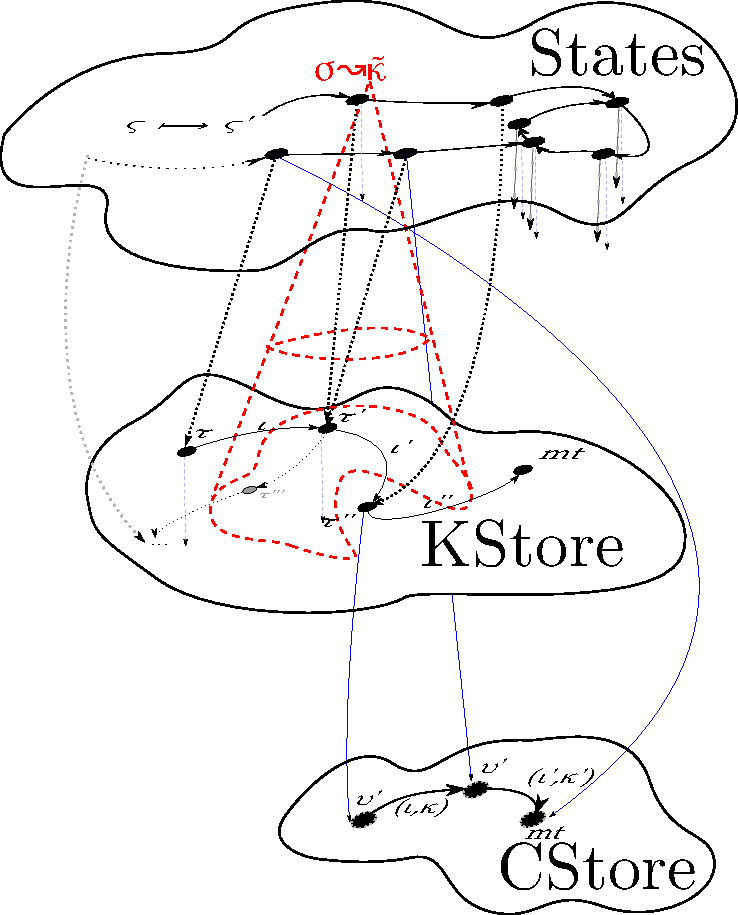
\includegraphics[scale=0.6]{xigraph-approx}
  \caption{Graphical visualization of states, $\mktab_{\makont}$ and $\mktab_{\mamkont}$.}
  \label{fig:shiftreset-vis}
\end{figure}

\begin{figure}
  \centering
  \begin{tabular}{rlrl}
    $\mastate \in \sa{SR}$ &\multicolumn{3}{l}{\hspace{-3mm}$::= \ev{\mexpr,\menv,\mastore,\mmktab,\makont,\mamkont} \alt \co{\makont,\mamkont,\maval,\mastore,\mmktab}$} \\
    $\State$ & \multicolumn{3}{l}{\hspace{-3mm}$::= \mastate,\mktab_{\makont},\mktab_{\mamkont}$} \\
    $\mmktab \in \MKTab$ &\multicolumn{3}{l}{\hspace{-3mm}$= \Addr \finto \wp(\Store)$} \\
    $\mktab_{\makont} \in \KStore$ &\multicolumn{3}{l}{\hspace{-3mm}$= \ExactContext \finto \wp(\sa{Kont})$} \\
    $\mktab_{\mamkont} \in \MKStore$ &\multicolumn{3}{l}{\hspace{-3mm}$= \MContext \finto \wp(\sa{Kont} \times \sa{MKont})$} \\
    $\makont \in \sa{Kont}$ &\hspace{-3mm}$::= \epsilon \alt \kcons{\mkframe}{\mctx} \alt \mctx$ & $\mvkont \in \VKont$ &\hspace{-3mm}$::= \epsilon \alt \mactx$ \\
    $\mamkont \in \sa{MKont}$ &\hspace{-3mm}$::= \epsilon \alt \mmctx$ & $\maval \in \sa{Value}$ &\hspace{-3mm}$::= \mvkont \alt (\mlam,\menv)$
  \end{tabular}
  \caption{Shift/reset abstract semantic spaces}
  \label{fig:shiftreset-spaces}
\end{figure}
%
The approximation and flattening happens in $\approximate$:
\begin{equation*}
  \approximate : \MKTab \times \Addr \times \SKont \to \MKTab \times \VKont
\end{equation*}
\begin{align*}
  \approximate(\mmktab,\maddr,\epsilon) &= \mmktab,\epsilon \\
  \approximate(\mmktab,\maddr,\kcons{\mkframe}{\mctx}) &= \mmktab',\kcons{\mkframe}{\mactx} \text{ where } (\mmktab',\mactx) = \approximate(\mmktab,\maddr,\mctx) \\
  \approximate(\mmktab,\maddr,\tpl{\mexpr,\menv,\mastore,\mmktab'}) &= \joinm{\mmktab\sqcup\mmktab'}{\maddr}{\mastore},\kcons{\mkframe}{\tpl{\mexpr,\menv,\maddr}} \\
  \approximate(\mmktab,\maddr,\tpl{\mexpr,\menv,\maddralt}) &= \joinm{\mmktab}{\maddr}{\mmktab(\maddralt)},\kcons{\mkframe}{\tpl{\mexpr,\menv,\maddr}}
\end{align*}
The third case is where continuation closures get flattened together.
%
The fourth case is when an already approximate continuation is approximated: the approximation is inherited.
%
Approximating the context and allocating the continuation in the store require two addresses, so we relax the specification of $\alloc$ to allow multiple address allocations in this case.

Each of the four rules of the original shift/reset machine has a corresponding rule that we explain piecemeal.
%
We will use $\kindastepto$ for steps that do not modify the continuation stores for notational brevity.
%
We use the above $\approximate$ function in the rule for continuation capture, as modified here.
%
\begin{equation*}\ev{\sshift{\mvar}{\mexpr},\menv,\mastore,\mmktab,\makont,\mamkont} \kindastepto
  \ev{\mexpr,\menv',\mastore',\mmktab',\epsilon,\mamkont}
\end{equation*}
where
\begin{align*}
  (\maddr,\maddr') &= \alloc(\mastate,\mktab_\makont,\mktab_\mamkont) & \menv' &= \extm{\menv}{\mvar}{\maddr} \\
  (\mmktab',\mvkont) &= \approximate(\mmktab,\maddr',\makont) &
  \mastore' &= \joinm{\mastore}{\maddr}{\mvkont}
\end{align*}

The rule for {\tt reset} stores the continuation and meta-continuation in $\mktab_{\mamkont}$:
\begin{align*}
\ev{\sreset{\mexpr},\menv,\mastore,\mmktab,\makont,\mamkont},\mktab_\makont,\mktab_\mamkont &\stepto
  \ev{\mexpr,\menv,\mastore,\mmktab,\epsilon,\mmctx},\mktab_\makont,\mktab_\mamkont' \\
  \text{where } \mmctx &= \tpl{\mexpr,\menv,\mastore,\mmktab} \\
                \mktab_\mamkont &= \joinm{\mktab_{\mamkont}}{\mmctx}{(\makont,\mamkont)}
\end{align*}

The prompt-popping rule simply dereferences $\mktab_{\mamkont}$:
\begin{align*}
  \co{\epsilon,\mmctx,\maval,\mastore,\mmktab} &\kindastepto \co{\makont,\mamkont,\maval,\mastore,\mmktab} \text{ if } (\makont,\mamkont) \in \mktab_{\mamkont}(\mmctx)
\end{align*}

The continuation installation rule extends $\mktab_{\mamkont}$ at the different context:
\begin{align*}
  \co{\makont,\mamkont,\maval,\mastore,\mmktab},\mktab_\makont,\mktab_\mamkont &\stepto \co{\mvkont,\mmctx,\maval,\mastore,\mmktab},\mktab_\makont,\mktab_\mamkont' \\ 
\text{if } & (\appr{\mvkont},\makont') \in \pop(\mktab_{\makont},\mmktab, \makont) \\
\text{where } \mmctx &= \tpl{\mvkont,\maval,\mastore,\mmktab} \\
              \mktab_\mamkont &= \joinm{\mktab_{\mamkont}}{\mmctx}{(\makont',\mamkont)}
\end{align*}
Again we have a metafunction $\pop$, but this time to interpret approximated continuations:
\begin{align*}
  \pop(\mktab_{\makont}, \mmktab, \makont) &= \popaux(\makont,\emptyset) \\
  \text{where } 
   \popaux(\epsilon, G) &= \emptyset \\
   \popaux(\kcons{\mkframe}{\mctx}, G) &= \set{(\mkframe,\mctx)} \\
   \popaux(\mctx, G) &= \bigcup\limits_{\makont \in G'}(\popaux(\makont, G\cup G')) \\
    \text{where } G' &= \bigcup\limits_{\msctx \in I(\mctx)}{\mktab_{\makont}(\msctx)} \setminus G \\
  I(\msctx) &= \set{\msctx} \\
  I(\tpl{\mexpr,\menv,\maddr}) &=
  \setbuild{\tpl{\mexpr,\menv,\mastore,\mmktab'} \in \dom(\mktab_{\makont})}
           {\mastore \in \mmktab(\maddr),
            \mmktab' \sqsubseteq \mmktab}
\end{align*}
Notice that since we flatten $\mmktab$s together, we need to compare for containment rather than for equality (in $I$).
%
A variant of this semantics with GC is available in the PLT redex models.

\paragraph{Comparison to CPS transform to remove {\tt shift} and {\tt reset}:}{
We lose precision if we use a CPS transform to compile away {\tt shift} and {\tt reset} forms, because variables are treated less precisely than continuations.
%
%In pushdown analysis, we track function return points with entire calling contexts rather than the $k$-CFA way of allocating the continuation in the heap at some lower-precision address, like a variable.
%
%In our summarizing analysis of delimited composable control, we get added precision for {\tt reset}, {\tt shift}, and continuation invocation points.
%
Consider the following program and its CPS transform for comparison:
% \begin{lstlisting}[mathescape]
% (let* ([id ($\lambda$ (x) x)]
%        [f ($\lambda$ (y) (shift k (k (k y))))]
%        [g ($\lambda$ (z) (reset (id (f z))))])
%   (<= (g 0) (g 1)))
% \end{lstlisting}
\begin{small}
\begin{SCodeFlow}\begin{RktBlk}\begin{SingleColumn}\RktPn{(}\RktSym{let*}\mbox{\hphantom{\Scribtexttt{x}}}\RktPn{(}\RktPn{[}\RktSym{id}\mbox{\hphantom{\Scribtexttt{x}}}\RktPn{(}\RktSym{$\lambda$}\mbox{\hphantom{\Scribtexttt{x}}}\RktPn{(}\RktSym{x}\RktPn{)}\mbox{\hphantom{\Scribtexttt{x}}}\RktSym{x}\RktPn{)}\RktPn{]}

\mbox{\hphantom{\Scribtexttt{xxxxxxx}}}\RktPn{[}\RktSym{f}\mbox{\hphantom{\Scribtexttt{x}}}\RktPn{(}\RktSym{$\lambda$}\mbox{\hphantom{\Scribtexttt{x}}}\RktPn{(}\RktSym{y}\RktPn{)}\mbox{\hphantom{\Scribtexttt{x}}}\RktPn{(}\RktSym{shift}\mbox{\hphantom{\Scribtexttt{x}}}\RktSym{k}\mbox{\hphantom{\Scribtexttt{x}}}\RktPn{(}\RktSym{k}\mbox{\hphantom{\Scribtexttt{x}}}\RktPn{(}\RktSym{k}\mbox{\hphantom{\Scribtexttt{x}}}\RktSym{y}\RktPn{)}\RktPn{)}\RktPn{)}\RktPn{)}\RktPn{]}

\mbox{\hphantom{\Scribtexttt{xxxxxxx}}}\RktPn{[}\RktSym{g}\mbox{\hphantom{\Scribtexttt{x}}}\RktPn{(}\RktSym{$\lambda$}\mbox{\hphantom{\Scribtexttt{x}}}\RktPn{(}\RktSym{z}\RktPn{)}\mbox{\hphantom{\Scribtexttt{x}}}\RktPn{(}\RktSym{reset}\mbox{\hphantom{\Scribtexttt{x}}}\RktPn{(}\RktSym{id}\mbox{\hphantom{\Scribtexttt{x}}}\RktPn{(}\RktSym{f}\mbox{\hphantom{\Scribtexttt{x}}}\RktSym{z}\RktPn{)}\RktPn{)}\RktPn{)}\RktPn{)}\RktPn{]}\RktPn{)}

\mbox{\hphantom{\Scribtexttt{xx}}}\RktPn{(}\RktSym{$\le$}\mbox{\hphantom{\Scribtexttt{x}}}\RktPn{(}\RktSym{g}\mbox{\hphantom{\Scribtexttt{x}}}\RktVal{0}\RktPn{)}\mbox{\hphantom{\Scribtexttt{x}}}\RktPn{(}\RktSym{g}\mbox{\hphantom{\Scribtexttt{x}}}\RktVal{1}\RktPn{)}\RktPn{)}\RktPn{)}\end{SingleColumn}\end{RktBlk}\end{SCodeFlow}

% \begin{lstlisting}[mathescape]
% (let* ([id ($\lambda$ (x k) (k x))]
%        [f ($\lambda$ (y j) (j (j y)))]
%        [g ($\lambda$ (z h) (h (f z ($\lambda$ (fv) (id fv ($\lambda$ (i) i))))))])
%   (g 0 ($\lambda$ (g0v) (g 1 ($\lambda$ (g1v) (<= g0v g1v))))))
% \end{lstlisting}
\begin{SCodeFlow}\begin{RktBlk}\begin{SingleColumn}\RktPn{(}\RktSym{let*}\mbox{\hphantom{\Scribtexttt{x}}}\RktPn{(}\RktPn{[}\RktSym{id}\mbox{\hphantom{\Scribtexttt{x}}}\RktPn{(}\RktSym{$\lambda$}\mbox{\hphantom{\Scribtexttt{x}}}\RktPn{(}\RktSym{x}\mbox{\hphantom{\Scribtexttt{x}}}\RktSym{k}\RktPn{)}\mbox{\hphantom{\Scribtexttt{x}}}\RktPn{(}\RktSym{k}\mbox{\hphantom{\Scribtexttt{x}}}\RktSym{x}\RktPn{)}\RktPn{)}\RktPn{]}

\mbox{\hphantom{\Scribtexttt{xxxxxxx}}}\RktPn{[}\RktSym{f}\mbox{\hphantom{\Scribtexttt{x}}}\RktPn{(}\RktSym{$\lambda$}\mbox{\hphantom{\Scribtexttt{x}}}\RktPn{(}\RktSym{y}\mbox{\hphantom{\Scribtexttt{x}}}\RktSym{j}\RktPn{)}\mbox{\hphantom{\Scribtexttt{x}}}\RktPn{(}\RktSym{j}\mbox{\hphantom{\Scribtexttt{x}}}\RktPn{(}\RktSym{j}\mbox{\hphantom{\Scribtexttt{x}}}\RktSym{y}\RktPn{)}\RktPn{)}\RktPn{)}\RktPn{]}

\mbox{\hphantom{\Scribtexttt{xxxxxxx}}}\RktPn{[}\RktSym{g}\mbox{\hphantom{\Scribtexttt{x}}}\RktPn{(}\RktSym{$\lambda$}\mbox{\hphantom{\Scribtexttt{x}}}\RktPn{(}\RktSym{z}\mbox{\hphantom{\Scribtexttt{x}}}\RktSym{h}\RktPn{)}
\\\mbox{\hphantom{\Scribtexttt{xxxxxxxxxxx}}}\RktPn{(}\RktSym{h}\mbox{\hphantom{\Scribtexttt{x}}}\RktPn{(}\RktSym{f}\mbox{\hphantom{\Scribtexttt{x}}}\RktSym{z}\mbox{\hphantom{\Scribtexttt{x}}}\RktPn{(}\RktSym{$\lambda$}\mbox{\hphantom{\Scribtexttt{x}}}\RktPn{(}\RktSym{fv}\RktPn{)}
\\\mbox{\hphantom{\Scribtexttt{xxxxxxxxxxxxxxxxxxxx}}}\RktPn{(}\RktSym{id}\mbox{\hphantom{\Scribtexttt{x}}}\RktSym{fv}\mbox{\hphantom{\Scribtexttt{x}}}\RktPn{(}\RktSym{$\lambda$}\mbox{\hphantom{\Scribtexttt{x}}}\RktPn{(}\RktSym{i}\RktPn{)}\mbox{\hphantom{\Scribtexttt{x}}}\RktSym{i}\RktPn{)}\RktPn{)}\RktPn{)}\RktPn{)}\RktPn{)}\RktPn{)}\RktPn{]}\RktPn{)}

\mbox{\hphantom{\Scribtexttt{xx}}}\RktPn{(}\RktSym{g}\mbox{\hphantom{\Scribtexttt{x}}}\RktVal{0}\mbox{\hphantom{\Scribtexttt{x}}}\RktPn{(}\RktSym{$\lambda$}\mbox{\hphantom{\Scribtexttt{x}}}\RktPn{(}\RktSym{g0v}\RktPn{)}\mbox{\hphantom{\Scribtexttt{x}}}\RktPn{(}\RktSym{g}\mbox{\hphantom{\Scribtexttt{x}}}\RktVal{1}\mbox{\hphantom{\Scribtexttt{x}}}\RktPn{(}\RktSym{$\lambda$}\mbox{\hphantom{\Scribtexttt{x}}}\RktPn{(}\RktSym{g1v}\RktPn{)}\mbox{\hphantom{\Scribtexttt{x}}}\RktPn{(}\RktSym{$\le$}\mbox{\hphantom{\Scribtexttt{x}}}\RktSym{g0v}\mbox{\hphantom{\Scribtexttt{x}}}\RktSym{g1v}\RktPn{)}\RktPn{)}\RktPn{)}\RktPn{)}\RktPn{)}\RktPn{)}\end{SingleColumn}\end{RktBlk}\end{SCodeFlow}
\end{small}
The $\CESKKstart$ machine with a monovariant allocation strategy will predict the CPS'd version returns true or false.
%
In analysis literature, ``monovariant'' means variables get one address, namely themselves.
%
Our specialized analysis for delimited control will predict the non-CPS'd version returns true.}

\iftr{
\subsection{Correctness}
We impose an order on values since stored continuations are more approximate in the analysis than in $\SR$:
\begin{mathpar}
  \inferrule{ }{\mval \sqsubseteq_{\mktab,\mmktab} \mval} \quad
  \inferrule{\mkont \sqsubseteq \unroll{\mktab,\mmktab}{\mvkont}}
            {\vcomp{\mkont} \sqsubseteq_{\mktab,\mmktab} \mvkont} \quad
  \inferrule{\forall \mval\in\mstore(\maddr).
             \exists \maval\in\mastore(\maddr).
             \mval \sqsubseteq_{\mktab,\mmktab} \maval}
            {\mstore \sqsubseteq_{\mktab,\mmktab} \mastore} \\
  \inferrule{\mkont \sqsubseteq \unroll{\mktab_{\makont},\mmktab}{\makont} \\
             \mmkont \sqsubseteq \unrollC{\mktab_{\makont},\mktab_{\mamkont},\mmktab}{\mamkont} \\
             \mstore \sqsubseteq_{\mktab_{\makont},\mmktab} \mastore}
            {\ev{\mexpr,\menv,\mstore,\mkont,\mmkont} \sqsubseteq
             \ev{\mexpr,\menv,\mastore, \mmktab,\makont,\mamkont}, \mktab_{\makont}, \mktab_{\mamkont}} \\
  \inferrule{\mval \sqsubseteq_{\mktab_{\makont},\mmktab} \maval \\
             \mkont \sqsubseteq \unroll{\mktab_{\makont},\mmktab}{\makont} \\
             \mmkont \sqsubseteq \unrollC{\mktab_{\makont},\mktab_{\mamkont},\mmktab}{\mamkont} \\
             \mstore \sqsubseteq_{\mktab_{\makont},\mmktab} \mastore}
            {\co{\mkont,\mmkont,\mval,\mstore} \sqsubseteq
             \co{\makont,\mamkont,\maval,\mastore, \mmktab}, \mktab_{\makont}, \mktab_{\mamkont}}
\end{mathpar}
Unrolling differs from the previous sections because the values in frames can be approximate.
%
Thus, instead of expecting the exact continuation to be in the unrolling, we have a judgment that an unrolling approximates a given continuation in \autoref{fig:cont-order} (note we reuse $I$ from $\popaux$'s definition).

\begin{figure}
  \centering
  \begin{mathpar}
    \inferrule{ }{\appl{\mexpr,\menv} \sqsubseteq_{\mktab,\mmktab}
      \appl{\mexpr,\menv}} \quad \inferrule{\mval
      \sqsubseteq_{\mktab,\mmktab}{\maval}}
    {\appr{\mval} \sqsubseteq_{\mktab,\mmktab} \appr{\maval}} \\
    \inferrule{ }{\epsilon \sqsubseteq
      \unroll{\mktab,\mmktab}{\epsilon}} \quad
    \inferrule{\mkframe \sqsubseteq_{\mktab,\mmktab} \makframe \\
      \mkont \sqsubseteq \unroll{\mktab,\mmktab}{\mctx}}
    {\kcons{\mkframe}{\mkont} \sqsubseteq
      \unroll{\mktab,\mmktab}{\kcons{\makframe}{\mctx}}}
    \\
    \inferrule{\makont \in \mktab(\msctx) \quad
      \mkont \sqsubseteq \unroll{\mktab,\mmktab}{\makont}} {\mkont
      \sqsubseteq \unroll{\mktab,\mmktab}{\msctx}}
    \quad
    \inferrule{\msctx \in I(\mktab,\mmktab,\mactx) \quad
      \mkont \sqsubseteq \unroll{\mktab,\mmktab}{\msctx}} {\mkont
      \sqsubseteq \unroll{\mktab,\mmktab}{\mactx}}
    \\
    \inferrule{ }
              {\epsilon \sqsubseteq \unrollC{\mktab_{\makont},\mktab_{\mamkont},\mmktab}{\epsilon}}
    \\
    \inferrule{(\makont,\mamkont) \in \mktab_{\mamkont}(\mmctx) \\
               \mkont \sqsubseteq \unroll{\mktab_{\makont},\mmktab}{\makont} \\
               \mmkont \sqsubseteq \unrollC{\mktab_{\makont},\mktab_{\mamkont},\mmktab}{\mamkont}}
              {\mkapp{\mkont}{\mmkont} \sqsubseteq \unrollC{\mktab_{\makont},\mktab_{\mamkont},\mmktab}{\mmctx}}
  \end{mathpar}
  
  \caption{Order on (meta-)continuations}
\label{fig:cont-order}
\end{figure}
\begin{theorem}[Soundness]
  If $\somestate \stepto_{\SR} \nextstate$, and $\somestate \sqsubseteq \someotherstate$ then there is $\nextotherstate$ such that $\someotherstate \stepto_{\SRSChKKt} \nextotherstate$ and
$\nextstate \sqsubseteq \nextotherstate$.
\end{theorem}

\paragraph{Freshness implies completeness}
The high level proof idea is that fresh allocation separates evaluation into a sequence of bounded length paths that have the same store, but the store only grows and distinguishes contexts such that each continuation and metacontinuation have a unique unrolling.
%
It is an open question whether the addition of garbage collection preserves completeness.
%
Each context with the same store will have different expressions in them since expressions can only get smaller until a function call, at which point the store grows.
%
This forms an order on contexts: smaller store means smaller context, and same store but smaller expression (indeed a subexpression) means a smaller context.
%
Every entry in each enviroment ($\mastore,\mmktab,\mktab_\makont,\mktab_\mamkont$) will map to a unique element, and the continuation stores will have no circular references (the context in the tail of a continuation is strictly smaller than the context that maps to the continuation).
%
There can only be one context that $I$ maps to for approximate contexts because of the property of stores in contexts.

We distill these intuitions into an invariant about states that we will then use to prove completeness.
%
\begin{mathpar}
  \inferrule{\forall \maddr\in\dom(\mastore).\exists \maval. \mastore(\maddr)=\set{\maval}\wedge\maval\preceq_\mmktab\mktab_\makont \\
    \forall \maddr\in\dom(\mmktab).\exists\mastore'.\mmktab(\maddr) =\set{\mastore'}\wedge\mastore'\in\pi_3(\dom(\mktab_\makont)) \\
    \forall \msctx\in\dom(\mktab_\makont).\exists\makont. \mktab_\makont(\msctx) = \set{\makont}\wedge \makont \sqsubset_\mmktab^{\mktab_\makont} \msctx\\
    \forall \mmctx\in\dom(\mktab_\mamkont).\exists\mamkont.\mktab_\mamkont(\mmctx) = \set{\mamkont}\wedge \mamkont \sqsubset \mmctx \\
}{\inv^*(\mastore, \mmktab, \mktab_{\makont}, \mktab_{\mamkont})}
 \\
\inferrule{\inv^*(\mastore,\mmktab,\mktab_\makont,\mktab_\mamkont) \\
           \tpl{\mexpr,\menv,\mastore,\mmktab} \sqsubset \dom(\mktab_\makont) \cup \dom(\mktab_\mamkont) \\
           (\exists \tpl{\mexpr_c,\menv,\mastore,\mmktab} \in \dom(\mktab_\makont)) \implies \mexpr \in \mathit{subexpressions}(\mexpr_c) \\
           \makont \preceq_\mmktab \mktab_\makont \\
           \mamkont \preceq \mktab_\mamkont}
          {\inv_\fresh(\ev{\mexpr,\menv,\mastore,\mmktab,\makont,\mamkont},\mktab_\makont,\mktab_\mamkont)} \\
\inferrule{\inv^*(\mastore,\mmktab,\mktab_\makont,\mktab_\mamkont) \\
           \maval \preceq_\mmktab \mktab_\makont \\
           \makont \preceq_\mmktab \mktab_\makont \\
           \mamkont \preceq \mktab_\mamkont}
          {\inv_\fresh(\co{\makont,\mamkont,\maval,\mastore,\mmktab},\mktab_\makont,\mktab_\mamkont)}
\end{mathpar}
Where the order $\preceq$ states that any contexts in the (meta-)continuation are mapped in the given table.
\begin{mathpar}
  \inferrule{ }{(\mlam,\menv) \preceq_\mmktab \mktab_\makont} \quad
  \inferrule{ }{\epsilon \preceq_\mmktab \mktab_\makont} \quad
  \inferrule{ }{\epsilon \preceq \mktab_\mamkont} \quad
  \inferrule{\msctx \in \dom(\mktab_\makont)}{\msctx\preceq_\mmktab \mktab_\makont} \quad
  \inferrule{\mmctx \in \dom(\mktab_\mamkont)}{\mmctx \preceq \mktab_\mamkont}\\
  \inferrule{\exists\mastore.\mmktab(\maddr)=\set{\mastore} \\
             \exists!\mmktab'.\tpl{\mexpr,\menv,\mastore,\mmktab'} \in\dom(\mktab_\makont)\wedge\mmktab' \sqsubseteq \mmktab
           }
            {\tpl{\mexpr,\menv,\maddr} \preceq_\mmktab \mktab_\makont}
\end{mathpar}
And the order $\sqsubset$ states that the contexts in the (meta-)continuation are strictly smaller than the given context.
\begin{mathpar}
  \inferrule{ }{\epsilon \sqsubset_\mmktab^{\mktab_{\makont}}} \quad \inferrule{ }{\epsilon \sqsubset \mmctx} \quad \inferrule{\mctx \sqsubset_\mmktab^{\mktab_\makont} \msctx}{\kcons{\mkframe}{\mctx} \sqsubset_\mmktab^{\mktab_\makont} \msctx} \\
  \inferrule{\mexpr' \in \mathit{subexpressions}(\mexpr)}{\tpl{\mexpr',\menv,\mastore,\mmktab} \sqsubset_\mmktab^{\mktab_\makont} \tpl{\mexpr,\menv,\mastore,\mmktab}} \quad
  \inferrule{\mexpr' \in \mathit{subexpressions}(\mexpr)}{\tpl{\mexpr',\menv,\mastore,\mmktab} \sqsubset \tpl{\mexpr,\menv,\mastore,\mmktab}} \\
  \inferrule{\dom(\mastore) \sqsubset \dom(\mastore')}{\tpl{\_,\_,\mastore,\_} \sqsubset_\mmktab^{\mktab_\makont} \tpl{\_,\_,\mastore',\_}} \quad
  \inferrule{\dom(\mastore) \sqsubset \dom(\mastore')}{\tpl{\_,\_,\mastore,\_} \sqsubset \tpl{\_,\_,\mastore',\_}} \\
  \inferrule{\forall \msctx' \in I(\mktab_\makont,\mmktab,\mactx) \\ \msctx' \sqsubset_\mmktab^{\mktab_\mkont} \msctx}{\mactx \sqsubset_\mmktab^{\mktab_\makont} \msctx}
\end{mathpar}

\begin{lemma}[Freshness invariant]
  If $\alloc$ produces fresh addresses, $\inv_{\fresh}(\mastate,\mktab_\makont,\mktab_\mamkont)$ and
$\mastate,\mktab_{\makont},\mktab_{\mamkont} \stepto
\mastate',\mktab'_{\makont},\mktab'_{\mamkont}$ then
$\inv_{\fresh}(\mastate',\mktab'_{\makont},\mktab'_{\mamkont})$.
\end{lemma}
\begin{proof}
  By case analysis on the step.
\end{proof}
\begin{theorem}[Complete for fresh allocation]
  If $\alloc$ produces fresh addresses then the resulting semantics is complete with respect to states satisfying the invariant.
\end{theorem}
\begin{proof}[Proof sketch]
  By case analysis and use of the invariant to exploit the fact the unrollings are unique and the singleton codomains pigeon-hole the possible steps to only concrete ones.
\end{proof}
}
%  LocalWords:  pushdown storeable codomain AAM ianjohnson Kiselyov
%  LocalWords:  modularly parsers undelimited Biernacki ev al ntinue
%  LocalWords:  Composable dereferences metafunction timestamped
%  LocalWords:  timestamp codomains

\section{Short-circuiting via ``summarization''}\label{sec:memo}
All the semantics of previous sections have a performance weakness that many analyses share: unnecessary propagation.
%
Consider two portions of a program that do not affect one another's behavior.
%
Both can change the store, and the semantics will be unaware that the changes will not interfere with the other's execution.
%
The more possible stores there are in execution, the more possible contexts in which a function will be evaluated.
%
Multiple independent portions of a program may be reused with the same arguments and store contents they depend on, but changes to irrelevant parts of the store lead to redundant computation.
%
The idea of skipping from a change past several otherwise unchanged states to uses of the change is called ``sparseness'' in the literature~\citep{dvanhorn:Reif1977Symbolic,dvanhorn:Wegman1991Constant,dvanhorn:Oh2012Design}.
%

%
Memoization is a specialized instance of sparseness; the base stack may change, but the evaluation of the function does not, so given an already computed result we can jump straight to the answer.
%
We use the vocabulary of ``relevance'' and ``irrelevance'' so that future work can adopt the ideas of sparseness to reuse contexts in more ways.
%

Recall the core notion of irrelevance: if we have seen the results of a computation before from a different context, we can reuse them.
%
The semantic counterpart to this idea is a memo table that we extend when popping and appeal to when about to push.
%
This simple idea works well with a deterministic semantics, but the non-determinism of abstraction requires care.
%
In particular, memo table entries can end up mapping to multiple results, but not all results will be found at the same time.
%
Note the memo table space:
\begin{align*}
  \mmemo \in \Memo &= \Context \finto \wp(\Relevant) \\
  \Relevant &::= \tpl{\mexpr,\menv,\mstore}
\end{align*}
%
There are a few ways to deal with multiple results:
\begin{enumerate}
\item{rerun the analysis with the last memo table until the table doesn't change (expensive),}
\item{short-circuit to the answer but also continue evaluating anyway (negates most benefit of short-circuiting), or}
\item{use a frontier-based semantics like in \autoref{sec:eng-frontier} with global $\mktab$ and $\mmemo$, taking care to
    \begin{enumerate}
    \item{at memo-use time, still extend $\mktab$ so later memo table extensions will ``flow'' to previous memo table uses, and}
    \item{when $\mktab$ and $\mmemo$ are extended at the same context at the same time, also create states that act like the $\mmemo$ extension point also returned to the new continuations stored in $\mktab$.}
    \end{enumerate}}
\end{enumerate}

We will only discuss the final approach.
%
The same result can be achieved with a one-state-at-a-time frontier semantics, but we believe this is cleaner and more parallelizable.
%
Its second sub-point we will call the ``push/pop rendezvous.''
%
The rendezvous is necessary because there may be no later push or pop steps that would regularly appeal to either (then extended) table at the same context.
%
The frontier-based semantics then makes sure these pushes and pops find each other to continue on evaluating.
%
In pushdown and nested word automata literature, the push to pop short-circuiting step is called a ``summary edge'' or with respect to the entire technique, ``summarization.''
%
We find the memoization analogy appeals to programmers' and semanticists' operational intuitions.
%

%
A second concern for using memo tables is soundness.
%
Without the completeness property of the semantics, memoized results in, \eg{}, an inexactly GC'd machine, can have dangling addresses since the possible stacks may have grown to include addresses that were previously garbage.
%
These addresses would not be garbage at first, since they must be mapped in the store for the contexts to coincide, but during the function evaluation the addresses can become garbage.
%
If they are supposed to then be live, and are used (presumably they are reallocated post-collection), the analysis will miss paths it must explore for soundness.
%

\iftr{
Context-irrelevance is a property of the semantics \emph{without} continuation stores, so there is an additional invariant to that of \autoref{sec:pushdown} for the semantics with $\mktab$ and $\mmemo$: $\mmemo$ respects context irrelevance.
\begin{mathpar}
  \inferrule{\dom(\mmemo) \subseteq \dom(\mktab) \\
             \forall \mctx\equiv\tpl{\mexpr_c,\menv_c,\mstore_c} \in \dom(\mmemo),
                     \tpl{\mexpr_r,\menv_r,\mstore_r} \in \mmemo(\mctx), \\
                     \makont\in\mktab(\mctx),
                     \mkont\in\unroll{\mktab}{\makont}. \\
              \exists\mtrace\equiv\tpl{\mexpr_c,\menv_c,\mstore_c,\mkont} \stepto_{\CESKt}^* \tpl{\mexpr_r,\menv_r,\mstore_r,\mkont}. \hastail(\mtrace,\mkont)}
            {\inv_M(\mktab,\mmemo)}
\end{mathpar}
Inexact GC does \emph{not} respect context irrelevance for the same reasons it is not complete: some states are spurious, meaning some memo table entries will be spurious, and the expected path in the invariant will not exist.
%
The reason we use unrolled continuations instead of simply $\epsilon$ for this (balanced) path is precisely for stack inspection reasons.
}

 \begin{figure}
   \begin{center}
     $\mastate,\mktab,\mmemo \stepto
     \mastate',\mktab',\mmemo'$
     \begin{tabular}{r|l}
       \hline\vspace{-3mm}\\
       $\tpl{\sapp{\mexpri0}{\mexpri1},\menv,\mstore,\makont},\mktab,\mmemo$
       &
       $\tpl{\mexpri0,\menv,\mstore,\kcons{\appl{\mexpri1,\menv}}{\mctx}},\mktab,\mmemo$ \\
       & \quad if $\mctx \notin\dom(\mmemo)$, or \\
       &
       $\tpl{\mexpr',\menv',\mstore',\makont},\mktab',\mmemo$ \\
       & \quad if $\tpl{\mexpr',\menv',\mstore'} \in \mmemo(\mctx)$ \\
       where & $\mctx = \tpl{\sapp{\mexpri0}{\mexpri1},\menv,\mstore}$ \\
       & $\mktab' = \joinm{\mktab}{\mctx}{\makont}$
       \\
       $\tpl{\mval,\mstore,\kcons{\appr{\slam{\mvar}{\mexpr},\menv}}{\mctx}},\mktab,\mmemo$
       &
       $\tpl{\mexpr,\menv',\mstore',\makont},\mktab,\mmemo'$ if $\makont \in \mktab(\mctx)$ \\
       where & $\menv' = \extm{\menv}{\mvar}{\maddr}$ \\
       & $\mstore' = \joinm{\mstore}{\maddr}{\mval}$ \\
       & $\mmemo' = \joinm{\mmemo}{\mctx}{\tpl{\mexpr,\menv',\mstore'}}$
     \end{tabular}
   \end{center}
   \caption{Important memoization rules}
   \label{fig:memo}
 \end{figure}

The rules in \autoref{fig:memo} are the importantly changed rules from \autoref{sec:pushdown} that short-circuit to memoized results.
%
The technique looks more like memoization with a $\CESIKKstart$ machine, since the memoization points are truly at function call and return boundaries.
%
The $\pop$ function would need to also update $\mmemo$ if it dereferences through a context, but otherwise the semantics are updated \emph{mutatis mutandis}.

\begin{equation*}
  {\mathcal F}_{\mexpr}(S,R,F,\mktab,\mmemo) = (S \cup F, R \cup R', F'\setminus S, \mktab', \mmemo')
\end{equation*}
where

\begin{tabular}{rlrlrl}
  $I$ &
  \multicolumn{5}{l}{
    \hspace{-3mm}$=\bigcup\limits_{\mstate \in
      F}{\setbuild{(\tpl{\mstate,\mstate'}, \mktab',\mmemo')}{\mstate,\mktab,\mmemo
        \stepto \mstate',\mktab',\mmemo'}}$}
\\
   $R'$ &\hspace{-3mm}$= \pi_0 I$ & $\mktab'$ & \hspace{-3mm}$= \bigsqcup\pi_1 I$ & $\mmemo'$ & \hspace{-3mm}$= \bigsqcup\pi_2 I$ \\
   $\Delta\mktab$ &\hspace{-3mm}$= \mktab'\setminus\mktab$ & $\Delta\mmemo$ & \hspace{-3mm}$= \mmemo'\setminus\mmemo$ & & \\
   $F'$ &
   \multicolumn{5}{l}{
     \hspace{-3mm}$= \pi_1 R' \cup \{{\tpl{\mexpr,\menv,\mstore,\makont}} :
     {\mctx \in \dom(\Delta\mktab)\cap\dom(\Delta\mmemo).}$}
   \\ &\multicolumn{5}{l}{\hspace{-3mm}$\phantom{= \pi_1 R' \cup \{} \makont \in \Delta\mktab(\mctx),
       \tpl{\mexpr,\menv,\mstore} \in \Delta\mmemo(\mctx)\}$}
 \end{tabular}

The $\pi_i$ notation is for projecting out pairs, lifted over sets.
%
This worklist algorithm describes unambiguously what is meant by ``rendezvous.''
%
After stepping each state in the frontier, the differences to the $\mktab$ and $\mmemo$ tables are collected and then combined in $F'$ as calling contexts' continuations matched with their memoized results.
%


\iftr{
\begin{theorem}[Correctness]
Same property is the same as in \autoref{thm:global-pushdown}, where $\reify$ ignores the $\mmemo$ component.
\end{theorem}
The proof appeals to the invariant on $\mmemo$ whose proof involves an additional argument for the short-circuiting step that reconstructs the path from a memoized result using both context irrelevance and the table invariants.
}
%  LocalWords:  parallelizable pushdown automata summarization
%  LocalWords:  memoization memoized dereferences

\section{Related Work}
\paragraph{Pushdown models and memoization}
The idea of relating pushdown automata with memoization is not new.
%
In 1971, Stephen Cook~\citep{DBLP:conf/ifip/Cook71} devised a transformation to simulate 2-way (on a fixed input) \emph{deterministic} pushdown automata in time linear in the size of the input, that uses the same ``context irrelevance'' idea to skip from state $q$ seen before to a corresponding first state that produced a smaller stack than $q$ was seen with.
%
Such a state is an instance of what are called \emph{terminator} states.
%
A \emph{terminator} state is simply a state that performs a pop operation.
%
Six years later, Neil D. Jones~\citep{Jones:1977:NLT} simplified the transformation instead to \emph{interpret} a stack machine program to work \emph{on-the-fly} still on a deterministic machine, but with the same idea of using memo tables to remember corresponding terminator states.
%
Thirty-six years after that, at David Schmidt's Festschrift, Robert Gl\"uck extended the technique to two-way \emph{non-deterministic} pushdown automata, and showed that the technique can be used to recognize context-free languages in the standard ${\mathcal O}(n^3)$ time~\citep{DBLP:journals/corr/Gluck13}.
%
Gl\"uck's technique (as yet, correctness unproven) uses the meta-language's stack with a deeply recursive interpretation function to preclude the use of a frontier and something akin to $\mktab$\footnote{See \texttt{gluck.rkt} in supplementary materials for \autoref{fig:real-impl} in Gl\"uck's style}.
%
By exploring the state space \emph{depth-first}, the interpreter can find all the different terminators a state can reach one-by-one by destructively updating the memo table with the ``latest'' terminator found.
%
The trade-offs with this technique are that it does not obviously scale to first-class control, and the search can overflow the stack when interpreting moderate-sized programs.
%
We have not performed an extensive evaluation to test the latter point, however.
%
A minor disadvantage is that it is also not a fair evaluation strategy when allocation is unbounded.
%
The technique can nevertheless be a viable alternative for languages with simple control-flow mechanisms.
%
It has close similarities to ``Big-CFA2'' in Vardoulakis' dissertation~\citep{vardoulakis-diss12}.
%%

%%
\paragraph{CFA2, PDCFA and AAM}
The immediately related work is that of PDCFA \citep{dvanhorn:Earl2010Pushdown, dvanhorn:Earl2012Introspective}, CFA2~\citep{ianjohnson:vardoulakis-lmcs11, ianjohnson:Vardoulakis2011Pushdown}, and AAM~\citep{dvanhorn:VanHorn2010Abstracting}.
%
The stack frames in CFA2 that boost precision are an orthogonal feature that fit into our model as an \emph{irrelevant} component along with the stack, which we did not cover in detail due to space constraints.
%
The version of CFA2 that handles \rackett{call/cc} does not handle composable control, is dependent on a restricted CPS representation, and has untunable precision for first-class continuations.
%
Our semantics adapts to \rackett{call/cc} by removing the meta-continuation operations, and thus this work supersedes theirs; the machinery is in fact a strict generalization.
%
The extended version of PDCFA that inspects the stack to do garbage collection~\citep{dvanhorn:Earl2012Introspective} also fits into our model;
the addresses that the stack keeps alive can be accumulated by ``reading through'' the continuation table, building up the set of addresses in each portion of the stack that we come across.
%

Additional work was done to improve the performance of the AAM approach in \citet{ianjohnson:oaam:icfp2013} that can almost entirely be imported for the work in this paper.
%
The technique that does not apply is ``store counting'' for lean representation of the store component of states when there is a global abstract store, an assumption that does not hold for garbage collection.
%
Their implementation\footnote{\url{http://github.com/dvanhorn/oaam}} has pushdown modules that use the ideas in this paper.

%%
\paragraph{Stack inspection}
Stack inspecting flow analyses also exist, but operate on pre-constructed regular control-flow graphs~\citep{ianjohnson:bartoletti2004stack}, so the CFGs cannot be trimmed due to the extra information at construction time, leading to less precision.
%
Backward analyses for stack inspection also exist, with the same prerequisite~\citep{ianjohnson:DBLP:journals/sigplan/Chang06}.
%%

%%
\paragraph{Analysis of pushdown automata}
Pushdown models have existed in the first-order static analysis literature~\citep[Chapter 7]{local:muchnick:jones:flow-analysis:1981}\citep{ianjohnson:reps:pushdown:1995}, and the first-order model checking literature \citep{ianjohnson:bouajiani:esparza:pushdown:1997}, for some time.
%
These methods already assume a pushdown model as input, and constructing a model from a first-order program is trivial.
%
In the setting of higher-order functions and first-class control, model construction is an additional problem -- the one we solve here.
%
Additionally, the algorithms employed in these works expect a complete description of the model up front, rather than work with a modified \texttt{step} function (also called \texttt{post}), such as in ``on-the-fly'' model-checking algorithms for finite state systems~\citep{DBLP:conf/tacas/SchwoonE05}.
%%

%%
\paragraph{Derivation from abstract machines}
The trend of deriving static analyses from abstract machines does not stop at flow analyses.
%
The model-checking community showed how to check temporal logic queries for collapsible pushdown automata (CPDA), or equivalently, higher-order recursion schemes, by deriving the checking algorithm from the Krivine machine~\citep{ianjohnson:Salvati:2011:KMH:2027223.2027239}.
%
The expressiveness of CPDAs outweighs that of PDAs, but it is unclear how to adapt higher-order recursion schemes (HORS) to model arbitrary programming language features.
%
The method is strongly tied to the simply-typed call-by-name lambda calculus and depends on finite sized base-types.
%
%HORSs are a powerful abstraction target for which monadic second order logic (MSO) is decidable, but systematic constructions of models in HORS from arbitrary programming languages are still out of reach.

\section{Conclusion}
As the programming world continues to embrace behavioral values like functions and continuations, it becomes more important to import the powerful techniques pioneered by the first-order analysis and model-checking communities.
%
It is our view that systematic approaches to analysis construction are pivotal to scaling them to production programming languages.
%
We showed how to systematically construct executable concrete semantics that point-wise abstract to pushdown analyses of higher-order languages.
%
We bypass the automata theoretic approach so that we are not chained to a pushdown automaton to model features such as first-class composable control operators.
%
The techniques employed for pushdown analysis generalize gracefully to apply to non-pushdown models and give better precision than regular methods.

\balance
\bibliographystyle{plainnat}
\bibliography{bibliography}

\end{document}
